%%%%%%%%%%%%%%%%%%%%%%%%%%%%%%%%%%%%%%%%%
% American Geophysical Union (AGU)
% LaTeX Template
% Version 1.0 (3/6/13)
%
% This template has been downloaded from:
% http://www.LaTeXTemplates.com
%
% Original author:
% The AGUTeX class and agu-ps referencing style were created and are owned 
% by AGU: http://publications.agu.org/author-resource-center/author-guide/latex-formatting-toolkit/
%
% This template has been modified from the blank AGU template to include
% examples of how to insert content and drastically change commenting. The
% structural integrity is maintained as in the original blank template.
%
% Important notes: 
% This template retains extensive commenting from the AGU template. It is heavily 
% advised you read these comments and follow them in order to insure a speedy 
% submission process.
%
%%%%%%%%%%%%%%%%%%%%%%%%%%%%%%%%%%%%%%%%%

%%%%%%%%%%%%%%%%%%%%%%%%%%%%%%%%%%%%%%%%%%%%%%%%%%%%%%%%%%%%%%%%%%%%%%%%%%%%
% AGUtmpl.tex: this template file is for articles formatted with LaTeX2e,
% Modified March 2013
%
% This template includes commands and instructions
% given in the order necessary to produce a final output that will
% satisfy AGU requirements.
%
% PLEASE DO NOT USE YOUR OWN MACROS
% DO NOT USE \newcommand, \renewcommand, or \def.
%
% FOR FIGURES, DO NOT USE \psfrag or \subfigure.
%
%%%%%%%%%%%%%%%%%%%%%%%%%%%%%%%%%%%%%%%%%%%%%%%%%%%%%%%%%%%%%%%%%%%%%%%%%%%%
%
% All questions should be e-mailed to latex@agu.org.
%
%%%%%%%%%%%%%%%%%%%%%%%%%%%%%%%%%%%%%%%%%%%%%%%%%%%%%%%%%%%%%%%%%%%%%%%%%%%%

% Step 1: Set the \documentclass

% There are two options for article format: two column (default) and draft.

% PLEASE USE THE DRAFT OPTION TO SUBMIT YOUR PAPERS.
% The draft option produces double spaced output.

% Choose the journal abbreviation for the journal you are submitting to:

% jgrga	JOURNAL OF GEOPHYSICAL RESEARCH
% gbc	GLOBAL BIOCHEMICAL CYCLES
% grl		GEOPHYSICAL RESEARCH LETTERS
% pal	PALEOCEANOGRAPHY
% ras	RADIO SCIENCE
% rog	REVIEWS OF GEOPHYSICS
% tec	TECTONICS
% wrr	WATER RESOURCES RESEARCH
% gc		GEOCHEMISTRY, GEOPHYSICS, GEOSYSTEMS
% sw	SPACE WEATHER
% ms	JAMES
%
%
%
% (If you are submitting to a journal other than jgrga,
% substitute the initials of the journal for "jgrga" below.)

%\documentclass[grl]{AGUTeX}
\documentclass[draft,grl]{AGUTeX}

% To create numbered lines:

% If you don't already have lineno.sty, you can download it from http://www.ctan.org/tex-archive/macros/latex/contrib/ednotes/ (or search the internet for lineno.sty ctan), available at TeX Archive Network (CTAN). Take care that you always use the latest version.

% To activate the commands, uncomment \usepackage{lineno} and \linenumbers*[1]command, below:

%\usepackage{lineno}
%\linenumbers*[1]

%  To add line numbers to lines with equations:
%  \begin{linenomath*}
%  \begin{equation}
%  \end{equation}
%  \end{linenomath*}

%%%%%%%%%%%%%%%%%%%%%%%%%%%%%%%%%%%%%%%%%%%%%%%%%%%%%%%%%%%%%%%%%%%%%%%%%
% Figures and Tables

% DO NOT USE \psfrag or \subfigure commands.

%  Figures and tables should be placed AT THE END OF THE ARTICLE, after the references.

%  Uncomment the following command to include .eps files (comment out this line for draft format):
%\usepackage[dvips]{graphicx}
\usepackage{graphicx}

% Substitute one of the following for [dvips] above if you are using a different driver program and want to proof your illustrations on your machine:
% [xdvi], [dvipdf], [dvipsone], [dviwindo], [emtex], [dviwin],
% [pctexps],  [pctexwin],  [pctexhp],  [pctex32], [truetex], [tcidvi],
% [oztex], [textures]

% use math package
\usepackage{amsmath} 

%  Uncomment the following command to allow illustrations to print when using Draft:
\setkeys{Gin}{draft=false}

% See how to enter figures and tables at the end of the article, after references.

%----------------------------------------------------------------------------------------
%	RUNNING HEAD AND CORRESPONDING AUTHOR
%----------------------------------------------------------------------------------------

% Author names in capital letters:
\authorrunninghead{BAN ET AL.}

%------------------------------------------------

% Shorter version of title entered in capital letters:
\titlerunninghead{PRECIPITATION  ASSIMILATION}

%------------------------------------------------

% Corresponding author mailing address and e-mail address:
\authoraddr{Corresponding author: Dr. Xin Zhang, National Center for Atmospheric Research, P. O. Box 3000, Boulder, CO 80307. (xinzhang@ucar.edu)}

%----------------------------------------------------------------------------------------

\begin{document}

%----------------------------------------------------------------------------------------
%	TITLE
%----------------------------------------------------------------------------------------

\title{The impact of assimilating NCEP Stage IV Precipitation on analyses and short-range forecasts in WRFDA 4D-Var}
%----------------------------------------------------------------------------------------
%	AUTHORS AND AFFILIATIONS
%----------------------------------------------------------------------------------------

% Use \author{\altaffilmark{}} and \altaffiltext{}

% \altaffilmark will produce footnote; matching \altaffiltext will appear at bottom of page.

\authors{Junmei Ban,\altaffilmark{1}
Xin Zhang\altaffilmark{1}, and
Xiang-Yu Huang\altaffilmark{1}}

\altaffiltext{1}{National Center for Atmospheric Research, Boulder, Colorado, USA}

%----------------------------------------------------------------------------------------
%	ABSTRACT
%----------------------------------------------------------------------------------------

% Do NOT include any \begin...\end commands within the body of the abstract.

\begin{abstract}
The precipitation data assimilation is added to Weather Research and Forecasting Data Assimilation system using four-dimensional variational data assimilation approach. Four experiments over a 10-day period in June 2010 are conducted to assess the impact of precipitation assimilation on analyses and short-range forecasts. Results show that assimilating precipitation data together with conventional data has a positive impact on model fields, particularly the low level humidity, comparing to assimilate conventional data or precipitation data alone. It also improves the Gilbert Skill Score for precipitation forecasts.

\end{abstract}

%----------------------------------------------------------------------------------------
%	ARTICLE CONTENT
%----------------------------------------------------------------------------------------

% The body of the article must start with a \begin{article} command
% \end{article} must follow the references section, before the figures and tables.

\begin{article}

\section{Introduction}

In the past few decades, the assimilation of precipitation observations using four-dimensional variational data assimilation (4D-Var) has been developed to improve the model initial states, and hence, to improve the skill of short-range forecasts.
\citet{Zupanski} demonstrated the technical feasibility of the approach and showed an improvement of precipitation forecasts in mid-latitudes by using a regional National Meteorological Center (NMC) eta forecast model and an incomplete adjoint model. Later, studies \citep{Zou,Tsuyuki,Xiao,Guo,Zhangandliu} indicated that the precipitation assimilation using 4D-Var leads to a reduction in the spin-up time, improves the moisture distributions in model initial conditions and improves the skill of short-range forecasts. Some operational weather services also assimilate precipitation operationally using 4D-Var method to improve precipitation forecasts, including Japan Meteorological Agency (JMA) \citep{Koizumi} and European Centre for Medium-Range Weather Forecasts (ECMWF)  \citep{Lopez}. 

In order to assimilate precipitation data in 4D-Var, the tangent linear model (TLM) and adjoint model (ADM) should include moist process. The redeveloped WRF model's TLM and ADM (WRFPLUS) \citep{Zhang} contained both cumulus parameterization and large-scale condensation. Taking advantages of the redeveloped WRFPLUS, it is a natural extension to add the precipitation assimilation capability to the WRF Data Assimilation System (WRFDA) 4D-Var \citep{Barker,Huang}. This study for the first time assimilates precipitation observation in WRFDA 4D-Var and explores the impact of precipitation assimilation on analyses and subsequent forecasts. 
Four experiments have been conducted over a 10-day period from 1 to 10 June 2010. Observations used in assimilation  experiments are conventional data and National Center for Environmental Prediction (NCEP) Stage IV 6-hourly accumulated precipitation. The results are evaluated using the Model Evaluation Tool(MET).

%------------------------------------------------
\section{Observations and preprocessing}  
The precipitation observations to be assimilated in this paper are NCEP stage IV precipitation data, 
which are mosaics of regional multi-sensor analysis produced by National Weather Service (NWS) River Forecast Centers (RFCs) and manual quality control gets done at the RFCs \citep{LinMitchell}. Hourly, 6-hourly and 24-hourly precipitation data are available on National Center for Atmospheric Research (NCAR) Cooperative Distributed Interactive Atmospheric Catalog System (CODIAC) (http://data.eol.ucar.edu/codiac/dss/id=21.093). We choose 6-hourly precipitation data  instead of hourly for 6-hour assimilation window to better satisfy the 4D-Var linearity assumption. The 6-hourly precipitation observations had been converted into the WRFDA readable data format and the precipitation error is assigned to 2 mm which will be discussed in more detail in section 4.2. Observations with innovations greater than 5 times the assumed observation error standard deviation were rejected. Original 4km resolution data were thinned to experiment resolution 30km.

Conventional data used in this paper includes land surface, marine surface, radiosonde, pibal and aircraft reports from the Global Telecommunications System (GTS) which originated from a wide variety of sources, and it was downloaded from http://rda.ucar.edu/datasets/ds337.0/ . Quality control was also preformed as described above and the observation error statistics (obserr.txt) in WRFDA were used.

\section{Experiments design and verification methods}
\subsection{Experiments design}
A 10-day period from 0000 UTC 1 to 1200 UTC 10 June 2010 has been selected for running the experiments. This period is chosen because it is characterized by many precipitation events of both convective and stratiform nature. Advanced Research Weather Research and Forecasting model (ARW-WRF) \citep{Skamarock} is used as the forecast model. The integration domain of the model covers the North American continent and the surrounding oceans. The horizontal resolution is 30km and there are 40 vertical levels with the model top at 50hPa. The WRF Single-Moment 5-class Microphysics scheme (WSM5)  \citep{Hong}, the Kain-Fritsch cumulus convection scheme \citep{KainFristsch}, and the Yonsei University (YSU) boundary layer parameterization \citep{Hong2006} are used. 

Four experiments, CONTROL, GTS, RAIN and GTS+RAIN, are designed to investigate the impact of precipitation assimilation on analyses and forecasts. A 6-h spin-up run is conducted using NCEP Final Analysis with horizontal spatial resolution of 1.0 x 1.0 degree and the output from the spin-up is used as the initial condition of the COTROL experiment as well as the first guess field for the 4D-Var experiments. The CONTROL run is performed without data assimilation and serves as the benchmark for evaluating the assimilation experiments. The experiment GTS only assimilates conventional observations, while the experiment RAIN only assimilates precipitation data. The experiment GTS+RAIN assimilates both conventional and precipitation data. The NMC method \citep{ParrisDerber} in the WRFDA package is used for background error calculations. To reduce the computational cost, multi-incremental 4D-Var is used, where the innovation in outer loop is computed with a high-resolution nonlinear model (30 km) and the minimization in inner loop is done with a low-resolution linearized model (90 km). A more detailed description of multi-incremental 4D-Var can be found in \citet{Zhangandhuang}. 

\subsection{Verification methods}

The MET developed at Developmental Testbed Center \citep{Brown} is used to evaluate the analyses and forecasts. Two datasets have been used as references. One dataset is the upper air sounding observations, which is used to evaluate model winds, temperature, and relative humidity. Root-mean square errors (RMSEs) are used as the verification metric. The other dataset is the NCEP Stage IV precipitation data. The original precipitation accumulations are available on a 4-km resolution polar-stereographic grid. It has been regrided to 30 km lambert conformal grid before verification. We acquire 12-h, 18-h and 24-h accumulated precipitation by summing of NCEP Stage IV 6-h accumulated precipitation. After interpolating and summing, verifications are done by using a grid-to-grid comparison. The Gilbert Skill Score (GSS) \citep{Gilbert} is used as the precipitation verification metric. RMSEs and GSSs have been calculated for the entire 10-day period of the experiments.

%------------------------------------------------

\section{Results} 
\subsection{Impact on model variables}
In order to evaluate how model variables are affected by the precipitation assimilation, RMSEs are computed for wind speed, temperature and relative humidity on different pressure levels.  Figure 1 gives the vertical profiles of wind speed RMSEs for four experiments at analysis, 12-h and 24-h forecast.  At analysis time(Figure 1a), the RMSE of CONTROL is between 2.5 m s$^{-1}$ to 4.5 m s$^{-1}$ from 1000hpa to 100hpa. GTS has significant lower RMSE than CONTROL in all levels and the largest RMSE difference between them is about 1.1 m s$^{-1}$ at 200hpa.   For the RAIN experiment, the RMSE is close to CONTROL except at lower level where RAIN gives smaller error about 2.1 m s$^{-1}$.  It indicated that only assimilating precipitation data can reduce the lower level RMSE, but the influence to higher level is very  neutral. The wind speed RMSE of GTS+RAIN is almost overlapped with GTS at analysis time. It indicated that the conventional data play a dominate role in improving the vertical structure of the wind speed fields in GTS+RAIN at analysis time. For 12-h and 24-h forecasts(Figure 1b and 1c), although the wind speed RMSE of the four experiments are very close, the RMSEs of GTS+RAIN are smaller than other experiments in the middle and lower levels. 

The vertical profiles of the temperature RMSEs for all experiments are shown in Figure 2. Comparing to CONTROL, the RMSEs in GTS have been reduced at all levels for analyses, 12-h and 24-h forecasts (Figure 2a-c). The temperature RMSEs of RAIN are smallest at 925hpa and 1000hpa for analysis and forecasts, but it is larger than COTROL in heights above 850hpa. For the GTS+RAIN experiment, the low-level temperature RMSE is slightly improved comparing to GTS. 

The vertical profiles of the relative humidity RMSEs for all experiments are shown in Figure 3. The RMSE in GTS has been much reduced from CONTROL except at 1000hpa for 12-h and 24-h forecasts (Figure 3b,3c), where RAIN has positive impact on it. When combining the conventional data to precipitation assimilation, the RMSEs of relative humidity in GTS+RAIN significantly reduced at all levels. The result is consistent with \citet{Zou}, which pointed that a standard procedure for precipitation assimilation should include sufficient moisture-related data to reduces the model's freedom in adjusting the moisture field. For GTS+RAIN includes the moisture-related observation, it produces better results than only assimilating precipitation or conventional data.

\subsection{Impact on precipitation forecast}
When dealing with the new type of observations, it is very important to estimate the observations error. According to previous studies, many authors assigned the observation error of accumulated precipitation empirically according to their cases. For example, \citet{Zupanski} used an observed precipitation error of only 0.001 mm for 24-h accumulated precipitation. \citet{Zou} using 0.045mm for 3-h accumulated precipitation. \citet{Guo} used the error of 3 mm for 1-h accumulated precipitation. For the information about the observation error on the NCEP Stage IV precipitation data were not available, the sensitivity of the precipitation forecast to the choice of precipitation error in assimilation experiments was tested. We assigned a series of the observation error by the value of 1, 2, 3, 4mm for 6-h accumulated precipitation. Figure 4 shows the GSSs for 24-h accumulated precipitation using the different precipitation error in assimilation experiment. For a perfect forecast, GSS is 1. The results show that the GSS is the highest at the 1mm and 5mm thresholds when the precipitation assimilation experiment uses 1mm observation error. However, the advantage is disappeared when threshold is greater than 10mm.  It indicates that the improvement on the small or moderate rain area is limited if we employ a larger error like 4mm or a smaller error like 1mm. Therefore, 2 mm precipitation error for 6-h accumulated precipitation is used in RAIN and GTS+RAIN experiments.

Figure 5 shows the threshold series of the GSS for 6-h (Figure 5a), 12-h (Figure 5b), 18-h (Figure 5c) and 24-h (Figure 5d) accumulated precipitation for the experiments CONTROL, GTS, RAIN and GTS+RAIN. In Figure 5a-d, the GSS in CONTROL is lowest among four experiments, except 6-h precipitation forecast for the threshold lower than 7.5mm, where GTS is worse than CONTROL.  For 12-h, 18-h and 24-h accumulated precipitation forecasts(Figure 5b,c,d), the GSSs in GTS are better than CONTROL but worse than GTS+RAIN, and it should be noticed that the GSSs in GTS have slightly improved from CONTROL for the thresholds lower than 5mm. 
For the RAIN experiment, the GSS is much improved at 6-h accumulated precipitation(Figure 5a), but after 6-h integration the score is decreased and lower than GTS+RAIN (Figure 5b-d). On the whole, GTS+RAIN systematically improved the GSS scores comparing to the only assimilate precipitation or conventional data experiments. On the one hand, precipitation data in the GTS+RAIN experiment improve the precipitation forecasts especially on the small rain area where assimilating only conventional data produced neutral impact, on the other hand, conventional observations especially the moisture-related data in GTS+RAIN experiment constrains the arbitrarily adjusting of the moisture analysis in precipitation assimilation then improve the subsequent forecasts. 

\section{Conclusion}
In this study, we use WRFDA 4D-Var to assimilate precipitation data. A 10-day period with several precipitation events is selected to assess the impact of precipitation assimilation on short-range forecasts. Four experiments have been conducted: CONTROL� without assimilation; GTS � assimilation of conventional data only; RAIN � assimilation of precipitation data only; and GTS+RAIN� assimilation of both conventional and precipitation data. It is found that assimilating precipitation data together with conventional data improves the vertical profile of wind speed, temperature and relative humidity comparing to only assimilating conventional or precipitation data, especially for the low level relative humidity. The positive impact on moisture field in GTS+RAIN is very important, for it subsequently influences the latent heat release, alters the thermodynamic and dynamic structure of the atmosphere, and then make improvement on precipitation forecasts. A serial of precipitation observation error have been assigned to test the sensitivity of the precipitation forecast to the choice of observation error. An error of 2mm for 6-hour accumulated precipitation is found to be a suitable value for our case.
For the impact on precipitation forecasts, it indicated that assimilating conventional data and precipitation data complement each other in improving the precipitation forecasts skill. The results suggested that the quantitative precipitation forecast can be much improved when we assimilate both conventional and precipitation data.

%----------------------------------------------------------------------------------------
%	APPENDICES (OPTIONAL)
%----------------------------------------------------------------------------------------

%%%%%%%%%%%%%%%%%%%%%%%%%%%%%%%%
%% Optional Appendix goes here

% \appendix resets counters and redefines section heads
% but doesn't print anything.
% After typing  \appendix

% \section{Here Is Appendix Title}
% will show
% Appendix A: Here Is Appendix Title

%\appendix

%\section{Appendix Title}

%Vivamus magna enim, aliquet id cursus a, pharetra ut purus. Phasellus suscipit nisi iaculis mi vulputate id interdum velit dictum. Nam ullamcorper elit in lectus ultrices vitae volutpat massa gravida. Etiam sagittis commodo neque eget placerat. Sed et nisi faucibus metus interdum adipiscing id nec lacus. Donec ipsum diam, malesuada at euismod consectetur, placerat quis diam. Phasellus cursus semper viverra. Proin magna tortor, blandit in ultricies id, facilisis at nibh. Proin eu neque est. Etiam euismod auctor ante. Mauris mauris sem, tincidunt a placerat rutrum, porta id est. Aenean non velit porta eros condimentum facilisis at in nibh. Etiam cursus purus ut orci rhoncus sit amet semper eros porttitor. Etiam ac leo at ipsum tincidunt consequat ac non sapien. Aenean sed leo diam, venenatis pharetra odio.

%----------------------------------------------------------------------------------------
%	GLOSSARY OR NOTATION (OPTIONAL)
%----------------------------------------------------------------------------------------

%%%%%%%%%%%%%%%%%%%%%%%%%%%%%%%%%%%%%%%%%%%%%%%%%%%%%%%%%%%%%%%%
%
% Optional Glossary or Notation section, goes here
%
%%%%%%%%%%%%%%
% Glossary is only allowed in Reviews of Geophysics
% \section*{Glossary}
% \paragraph{Term}
% Term Definition here
%
%%%%%%%%%%%%%%
% Notation -- End each entry with a period.
% \begin{notation}
% Term & definition.\\
% Second term & second definition.\\
% \end{notation}
%%%%%%%%%%%%%%%%%%%%%%%%%%%%%%%%%%%%%%%%%%%%%%%%%%%%%%%%%%%%%%%%

%----------------------------------------------------------------------------------------
%	ACKNOWLEDGEMENTS
%----------------------------------------------------------------------------------------

\begin{acknowledgments}
The National Center for Atmospheric Research is sponsored by the National Science Foundation. This work is supported by the Air Force Weather Agency.
We thank John Halley Gotway and Tatiana Burek for their help with METViewer.
\end{acknowledgments}

%----------------------------------------------------------------------------------------
%	BIBLIOGRAPHY
%----------------------------------------------------------------------------------------

% Either type in your references using
% \begin{thebibliography}{}
% \bibitem{}
% Text
% \end{thebibliography}

% Or,

% If you use BiBTeX for your references, please use the agufull08.bst file (available at % ftp://ftp.agu.org/journals/latex/journals/Manuscript-Preparation/) to produce your .bbl
% file and copy the contents into your paper here.

% Follow these steps:
% 1. Run LaTeX on your LaTeX file.

% 2. Make sure the bibliography style appears as \bibliographystyle{agufull08}. Run BiBTeX on your LaTeX
% file.

% 3. Open the new .bbl file containing the reference list and
%   copy all the contents into your LaTeX file here.

% 4. Comment out the old \bibliographystyle and \bibliography commands.

% 5. Run LaTeX on your new file before submitting.

% AGU does not want a .bib or a .bbl file. Please copy in the contents of your .bbl file here.

\begin{thebibliography}{}

\providecommand{\natexlab}[1]{#1}
\expandafter\ifx\csname urlstyle\endcsname\relax
  \providecommand{\doi}[1]{doi:\discretionary{}{}{}#1}\else
  \providecommand{\doi}{doi:\discretionary{}{}{}\begingroup
  \urlstyle{rm}\Url}\fi

\bibitem[{\textit{Barker et~al.}(2012)}]{Barker}
Barker, D., et al. (2012), The weather research and forecasting (WRF) 
model's community variational/ensemble data assimilation system: WRFDA,
\textit{Bull. Amer. Meteor. Soc.}, \textit{56}(193), 119--139.

\bibitem[{\textit{Brown et~al.}(2009)}]{Brown}
Brown, B.~G., J.~H. Gotway, R. Bullock, E. Gilleland, and D. Ahijevych  (2009), 
Community tools for forecast evaluation,
\textit{25th Conf, Int. Interactive Information and Processing Systems(IIPS) for Meteororlogy}, Paper 9A.6.

\bibitem[{\textit{Gandin and Murphy}(1992)}]{Gilbert}
Gandin, L. S. and A. H. Murphy (1992),
Equitable Skill Scores for Categorical Forecasts.
\textit{Mon. Wea. Rev.}, \textit{120}, 361-370.

\bibitem[{\textit{Guo et~al.}(2000)}]{Guo}
Guo, Y.-R., Y.-H. Kuo, J. Dudhia, D. Parsons, and C. Rocken (2000), 
Four-dimensional variational assimilation of heterogeneous mesoscale 
observations for a strong convective case,
\textit{Mon. Wea. Rev.}, \textit{128}, 619-643.

\bibitem[{\textit{Hong et~al.}(2004)}]{Hong}
Hong, S.-Y., J. Dudhia, and S.-H. Chen (2004), 
A revised approach to ice microphysical processes for the bulk 
parameterization of clouds and precipitation,
\textit{Mon. Wea. Rev.}, \textit{132}, 103-120.

\bibitem[{\textit{Hong et~al.}(2006)}]{Hong2006}
Hong S.-Y., Y. Noh, and J. Dudhia (2006), 
A new vertical diffusion package with an explicit 
treatment of entrainment processes,
\textit{Mon. Wea. Rev.}, \textit{134}, 2318-2341.

\bibitem[{\textit{Huang et~al.}(2009)}]{Huang}
Huang, X.-Y., and coauthors (2009), 
Four-Dimensional Variational Data Assimilation for WRF: 
Formulation and Preliminary Results,
\textit{Mon. Wea. Rev.}, \textit{137}, 299-314.

\bibitem[{\textit{Kain and Fristsch}(1993)}]{KainFristsch}
Kain, J. S., and J. M. Fritsch (1990),
A one-dimensional entraining/detraining plume model and 
its application in convective parameterization,
\textit{J. Atmos. Sci.}, \textit{47}, 2784-2802.

\bibitem[{\textit{Koizumi et~al}(2005)}]{Koizumi}
Koizumi, K., Y. Ishikawa, and T. Tsuyuki (2005),
Assimilation of precipitation data to JMA mesoscale model with a four-dimensional variational method and its impact on precipitation forecasts.
\textit{SOLA}, \textit{1}, 45-48.

\bibitem[{\textit{Lin and Mitchell}(2005)}]{LinMitchell}
Lin, Y., and K.~E. Mitchell (2005), The NCEP stage II/IV hourly precipitation 
analyses: Development and applications,
 Preprints, \textit{8th Conf. on Mesoscale Processes}, Boulder, CO. pp341-344.

\bibitem[{\textit{Lopez}(2011)}]{Lopez}
Lopez P. (2011),
Direct 4D-Var Assimilation of NCEP Stage IV Radar and Gauge Precipitation Data at ECMWF.
\textit{Mon. Weather Rev.}, \textit{139}, 2098-2116.

\bibitem[{\textit{Macpherson}(2001)}]{Macpherson}
Macpherson, B. (2001),
Operational experience with assimilation of rainfall data in the Met Office mesoscale model. 
\textit{Meteor. Atmos. Phys.}, \textit{76}, 3-8.

\bibitem[{\textit{Parris and Derber}(1992)}]{ParrisDerber}
Parrish, D. F., and J. C. Derber (1992),
The National Meteorological Center�s spectral statistical-interpolation analysis system.
\textit{Mon. Weather Rev.}, \textit{120}, 1747-1763.

\bibitem[{\textit{Skamarock et~al.}(2008)}]{Skamarock}
Skamarock, W. C., J. B. Klemp, J. Dudhia, D. O. Gill, D. M. Barker, M. Duda, X. -Y. 
Huang, W. Wang, and J. G. Powers (2008),
A description of the advanced research WRF version 3, 
\textit{Meteor. Atmos. Phys.}, \textit{76}, 3-8.
NCAR Tech. Note TN-475+STR, 113 pp.

\bibitem[{\textit{Tsuyuki}(1996)}]{Tsuyuki}
Tsuyuki, T. (1996),
Variational data assimilation in the tropics using precipitation data Part I: column model. 
\textit{Meteor. Atmos. Phys.}, \textit{60}, 87-104.

\bibitem[{\textit{Tsuyuki}(1997)}]{Tsuyuki97}
Tsuyuki, T. (1997),
Variational data assimilation in the tropics using precipitation data Part III: assimilation of SSM/I precipitation rates. 
\textit{Meteor. Atmos. Phys.}, \textit{125}, 1447-1464.

\bibitem[{\textit{Xiao et~al.}(2000)}]{Xiao}
Xiao, Q., X. Zou and Y.-H. Kuo (2000),
Incorporating the SSM/I-derived precipitable water and rainfall rate into a numerical model: a case study for the ERICA IOP- 4 cyclone. 
\textit{Mon. Weather Rev.}, \textit{128}, 87-108.

\bibitem[{\textit{Xu et~al.}(2006)}]{Xu}
Xu, J., Q. Xiao, X. Gao, and S. Sorooshian (2006),
Influence of assimilating rainfall derived from WSR-88D radar on the rainstorm forecasts over the southwestern United States.
\textit{J. Geophys. Res.}, \textit{111}, D13105, doi:10.1029/2005JD006650.

\bibitem[{\textit{Zhang et~al.}(2003)}]{Zhangandliu}
Zhang, X., Y. Liu, B. Wang, and Z. Ji  (2003), 
Four-dimensional variational assimilation using rainfall observation in heavy rain simulation. 
\textit{Prog. Nat. Sci.}, \textit{13}, 1329-1333.

\bibitem[{\textit{Zhang et~al.}(2013a)}]{Zhang}
Zhang, X., X.-Y. Huang, and N. Pan (2013a),
Development of the Upgraded Tangent Linear and Adjoint of the Weather Research and Forecasting (WRF) Model. 
\textit{J. Atmos. Oceanic Technol.}, \textit{30}, 1180-1118. doi:10.1175/JTECH-D-12-00213.1.

\bibitem[{\textit{Zhang et~al.}(2013b)}]{Zhangandhuang}
Zhang, X., X.-Y. Huang, J. Liu and J. Poterjoy (2013b),
Development of the Upgraded Tangent Linear and Adjoint of the Weather Research and Forecasting (WRF) Model. 
submitted to \textit{J. Atmos. Oceanic Technol.} 

\bibitem[{\textit{Zou and Kuo}(1996)}]{Zou}
Zou, X., and Y.-H. Kuo (1996),
Rainfall assimilation through an optimal control of initial and boundary conditions in a limited-area mesoscale model. 
\textit{Mon. Weather Rev.}, \textit{124}, 2859-2882.

\bibitem[{\textit{Zupanski and Mesinger}(1995)}]{Zupanski}
Zupanski, D., and F. Mesinger (1995),
Four-dimensional variational assimilation of precipitation data.
\textit{Mon. Weather Rev.}, \textit{123}, 1112-1127.

\end{thebibliography}

% Reference citation examples:

%...as shown by \textit{Kilby} [2008].
%...as shown by {\textit  {Lewin}} [1976], {\textit  {Carson}} [1986], {\textit  {Bartholdy and Billi}} [2002], and {\textit  {Rinaldi}} [2003].
%...has been shown [\textit{Kilby et al.}, 2008].
%...has been shown [{\textit  {Lewin}}, 1976; {\textit  {Carson}}, 1986; {\textit  {Bartholdy and Billi}}, 2002; {\textit  {Rinaldi}}, 2003].
%...has been shown [e.g., {\textit  {Lewin}}, 1976; {\textit  {Carson}}, 1986; {\textit  {Bartholdy and Billi}}, 2002; {\textit  {Rinaldi}}, 2003].

%...as shown by \citet{jskilby}.
%...as shown by \citet{lewin76}, \citet{carson86}, \citet{bartoldy02}, and \citet{rinaldi03}.
%...has been shown \citep{jskilbye}.
%...has been shown \citep{lewin76,carson86,bartoldy02,rinaldi03}.
%...has been shown \citep [e.g.,][]{lewin76,carson86,bartoldy02,rinaldi03}.

% Please use ONLY \citet and \citep for reference citations.
% DO NOT use other cite commands (e.g., \cite, \citeyear, \nocite, \citealp, etc.).

\end{article}

%----------------------------------------------------------------------------------------
%	FIGURES AND TABLES
%----------------------------------------------------------------------------------------

%% Enter Figures and Tables here:
%
% DO NOT USE \psfrag or \subfigure commands.
%
% Figure captions go below the figure.
% Table titles go above tables; all other caption information should be placed in footnotes below the table.
%
%----------------
% EXAMPLE FIGURE
%
% \begin{figure}
% \noindent\includegraphics[width=20pc]{samplefigure.eps}
% \caption{Caption text here}
% \label{figure_label}
% \end{figure}
%
% ---------------
% EXAMPLE TABLE
%
%\begin{table}
%\caption{Time of the Transition Between Phase 1 and Phase 2\tablenotemark{a}}
%\centering
%\begin{tabular}{l c}
%\hline
% Run  & Time (min)  \\
%\hline
%  $l1$  & 260   \\
%  $l2$  & 300   \\
%  $l3$  & 340   \\
%  $h1$  & 270   \\
%  $h2$  & 250   \\
%  $h3$  & 380   \\
%  $r1$  & 370   \\
%  $r2$  & 390   \\
%\hline
%\end{tabular}
%\tablenotetext{a}{Footnote text here.}
%\end{table}

% See below for how to make sideways figures or tables.

\newpage
\begin{figure}
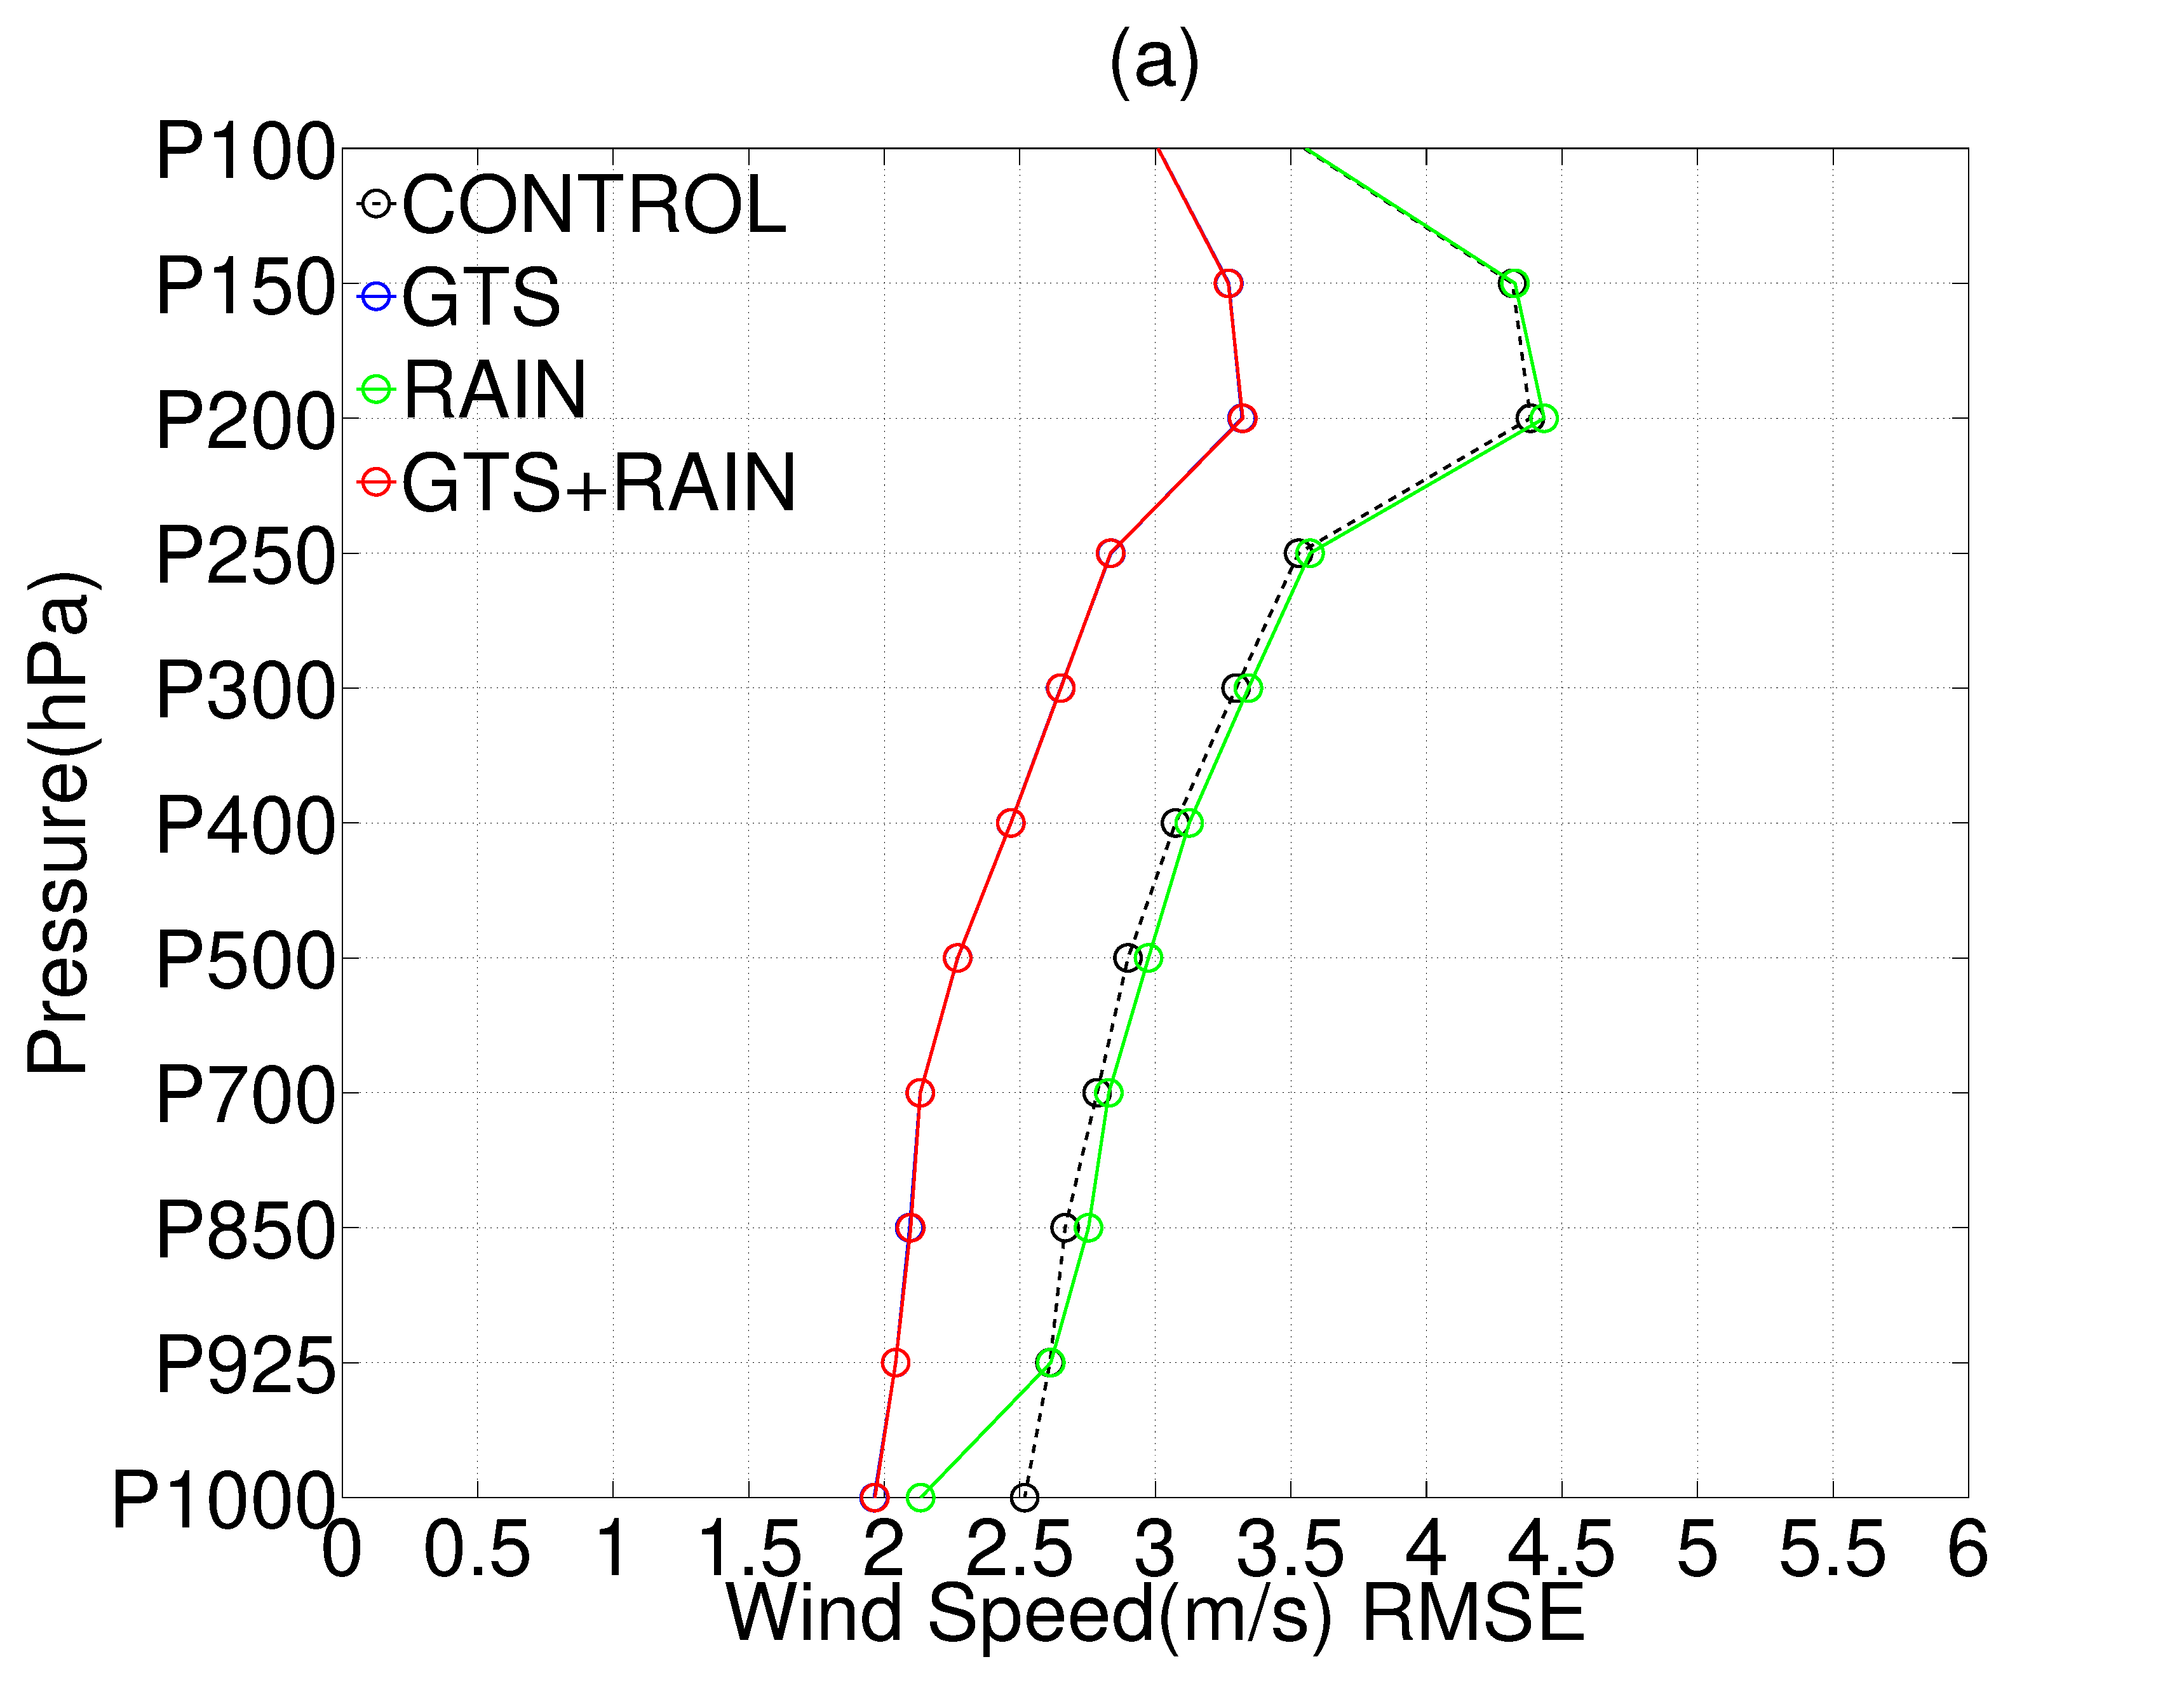
\includegraphics[width=0.45\linewidth]{./figures/wind_00.eps}

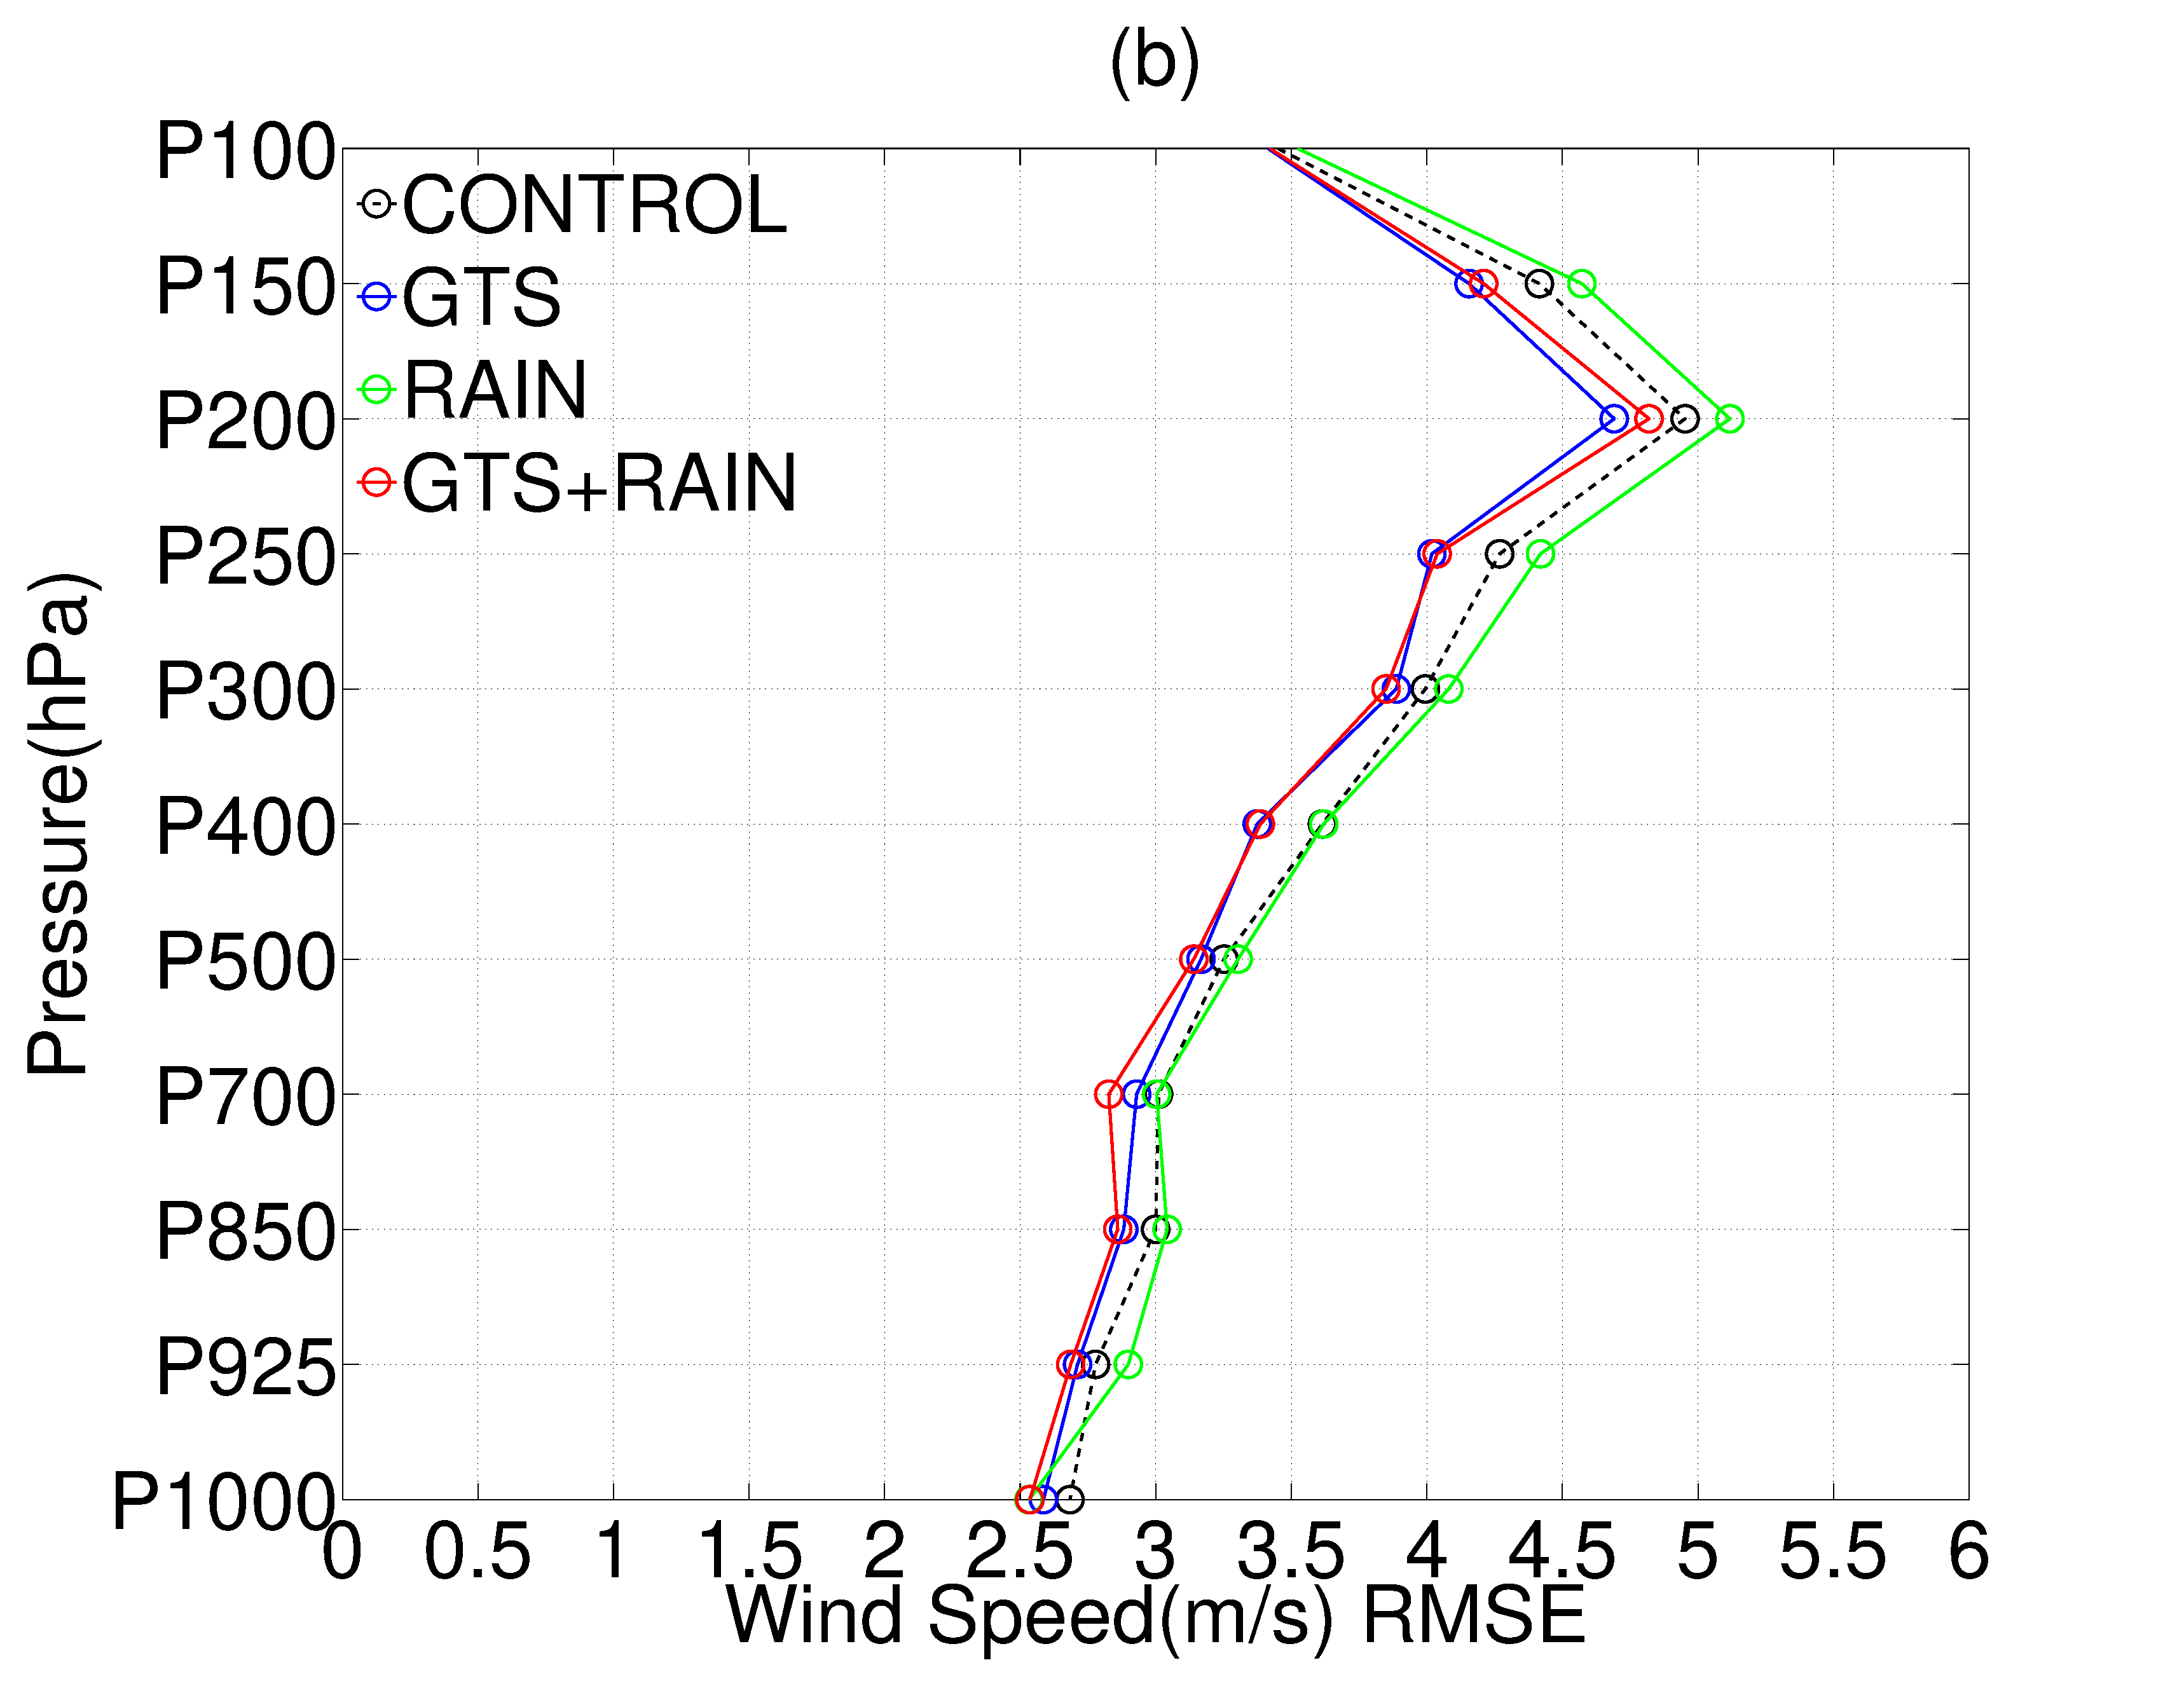
\includegraphics[width=0.45\linewidth]{./figures/wind_12.eps}

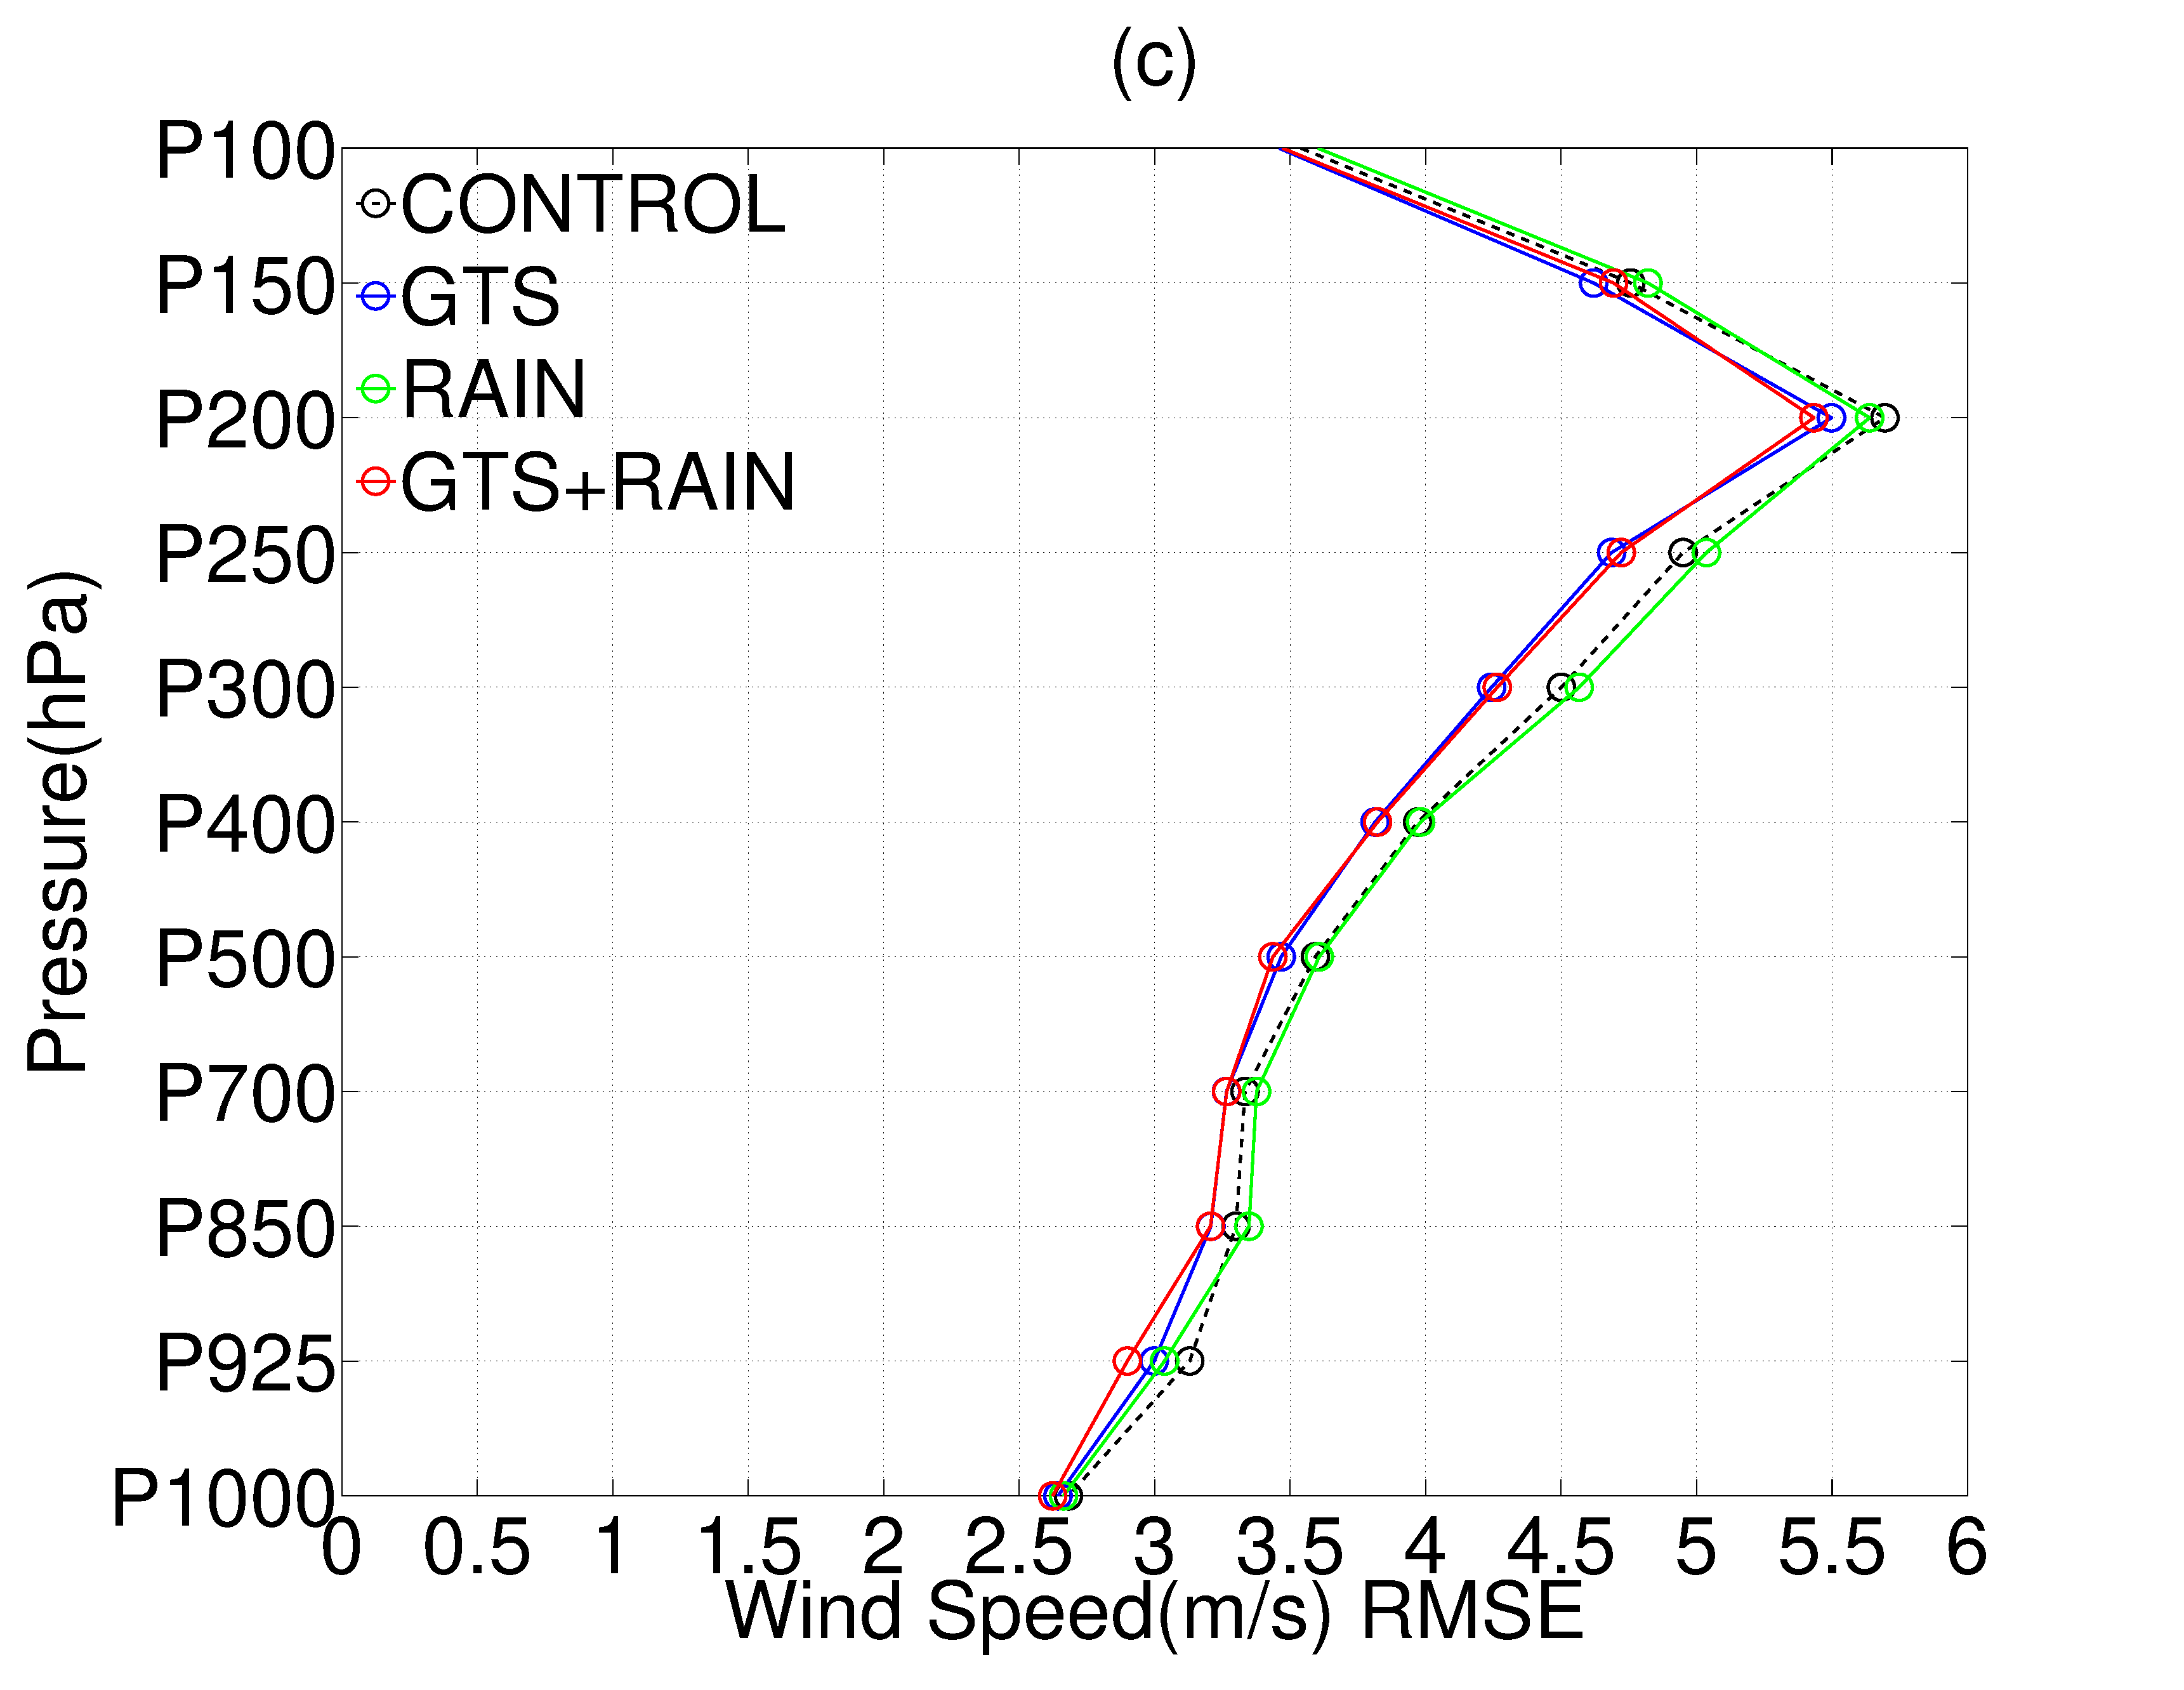
\includegraphics[width=0.45\linewidth]{./figures/wind_24.eps}
\caption{Vertical profiles of the RMSEs of wind speed for experiments CONTROL, GTS, RAIN and GTS+RAIN for analysis (a), 12-h forecast(b) and 24-h forecast(c) aggregated over 10-day period of the case verified against upper air sounding data.}\label{u_00}
\end{figure}


\newpage
\begin{figure}
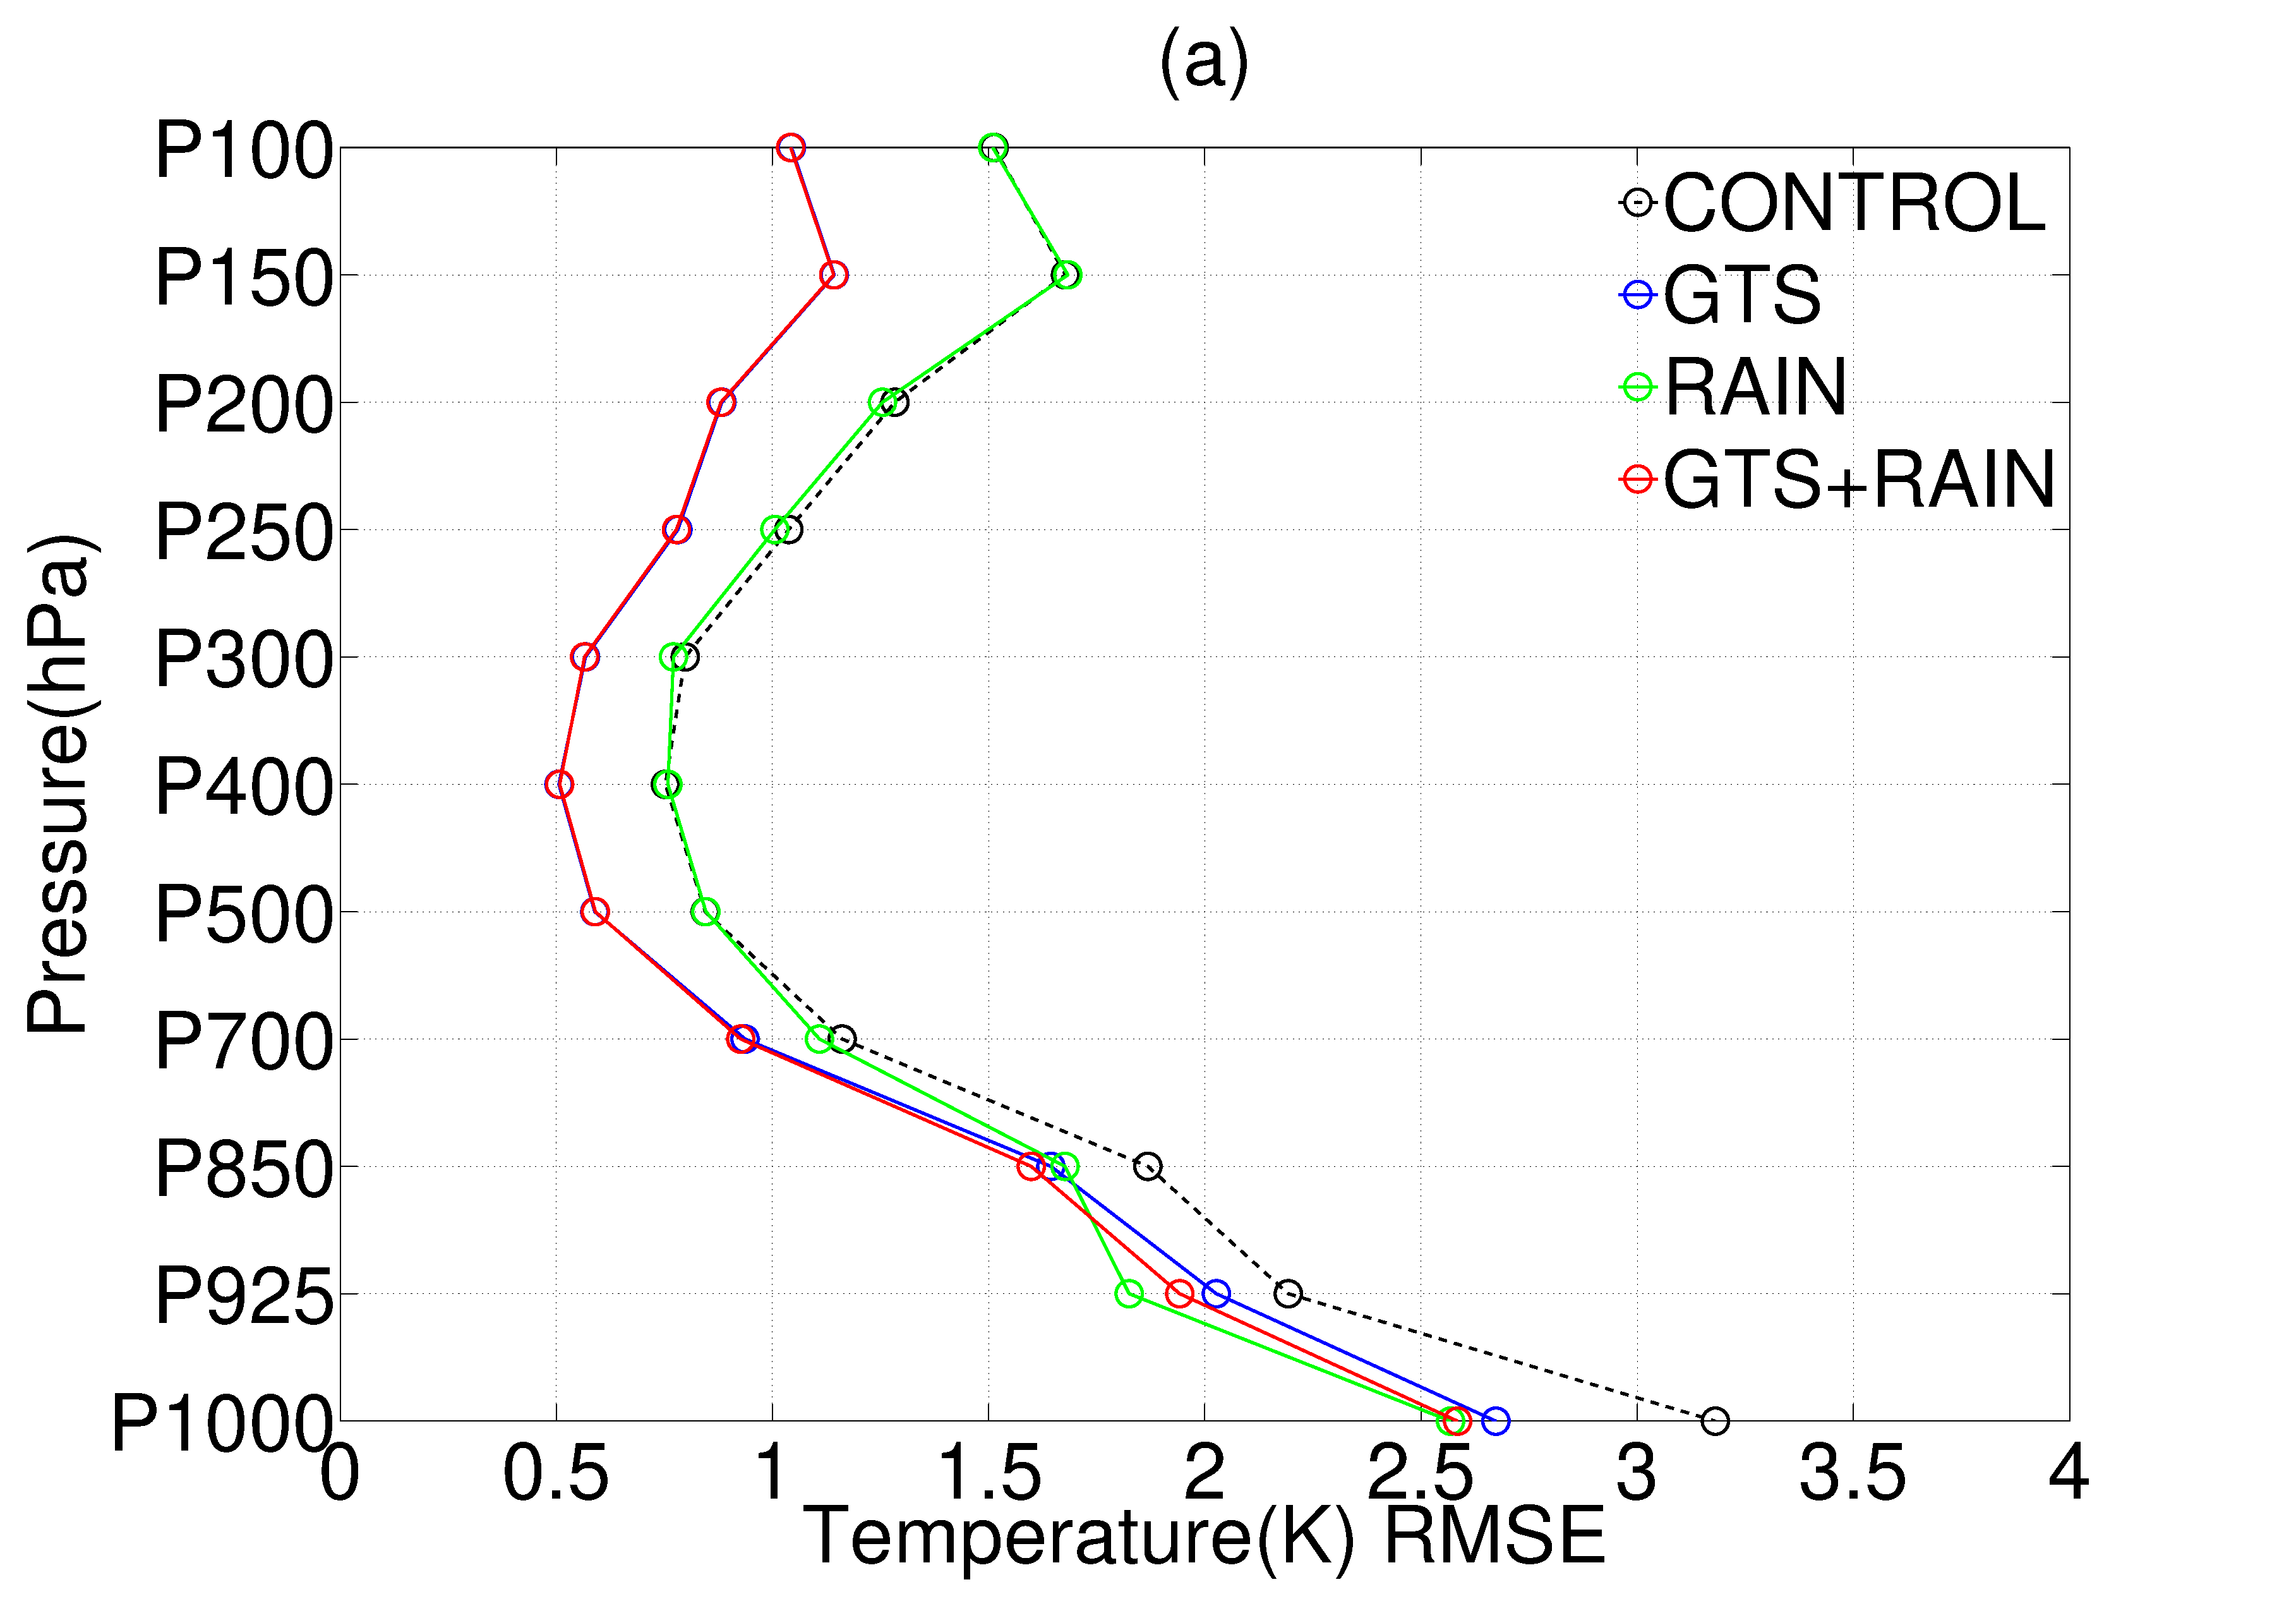
\includegraphics[width=0.5\linewidth]{./figures/tmp_00.eps}

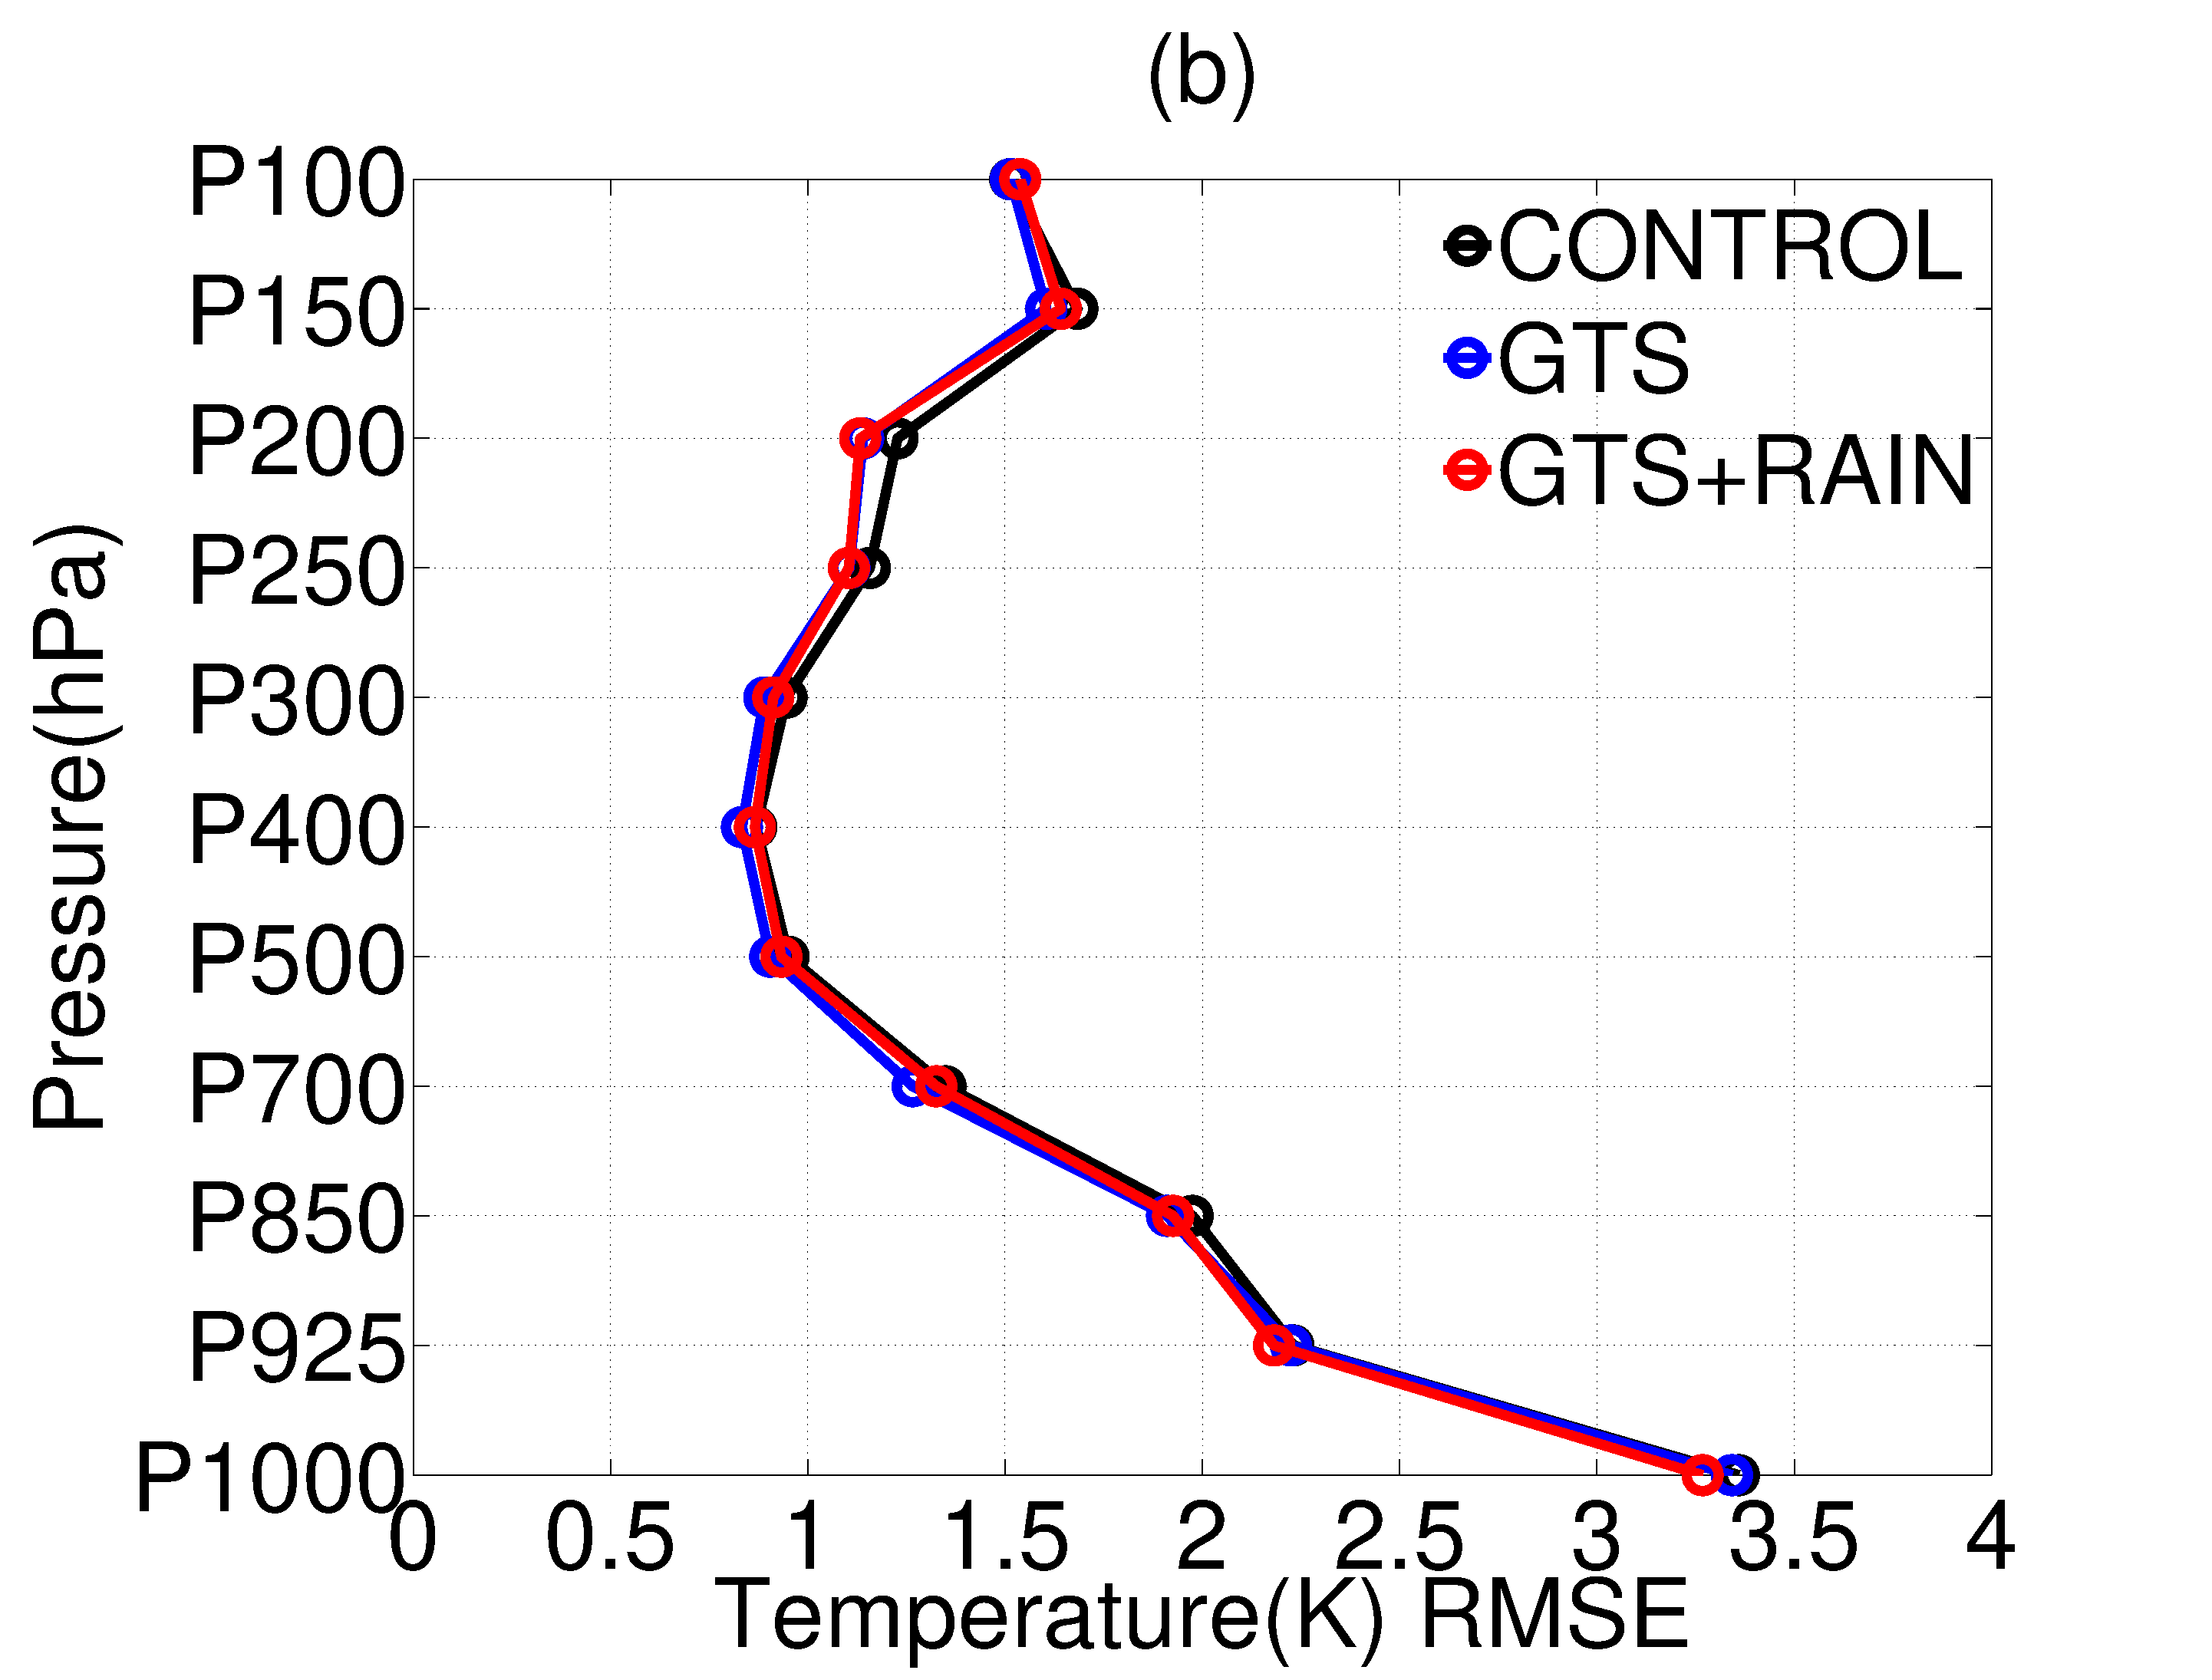
\includegraphics[width=0.5\linewidth]{./figures/tmp_12.eps}

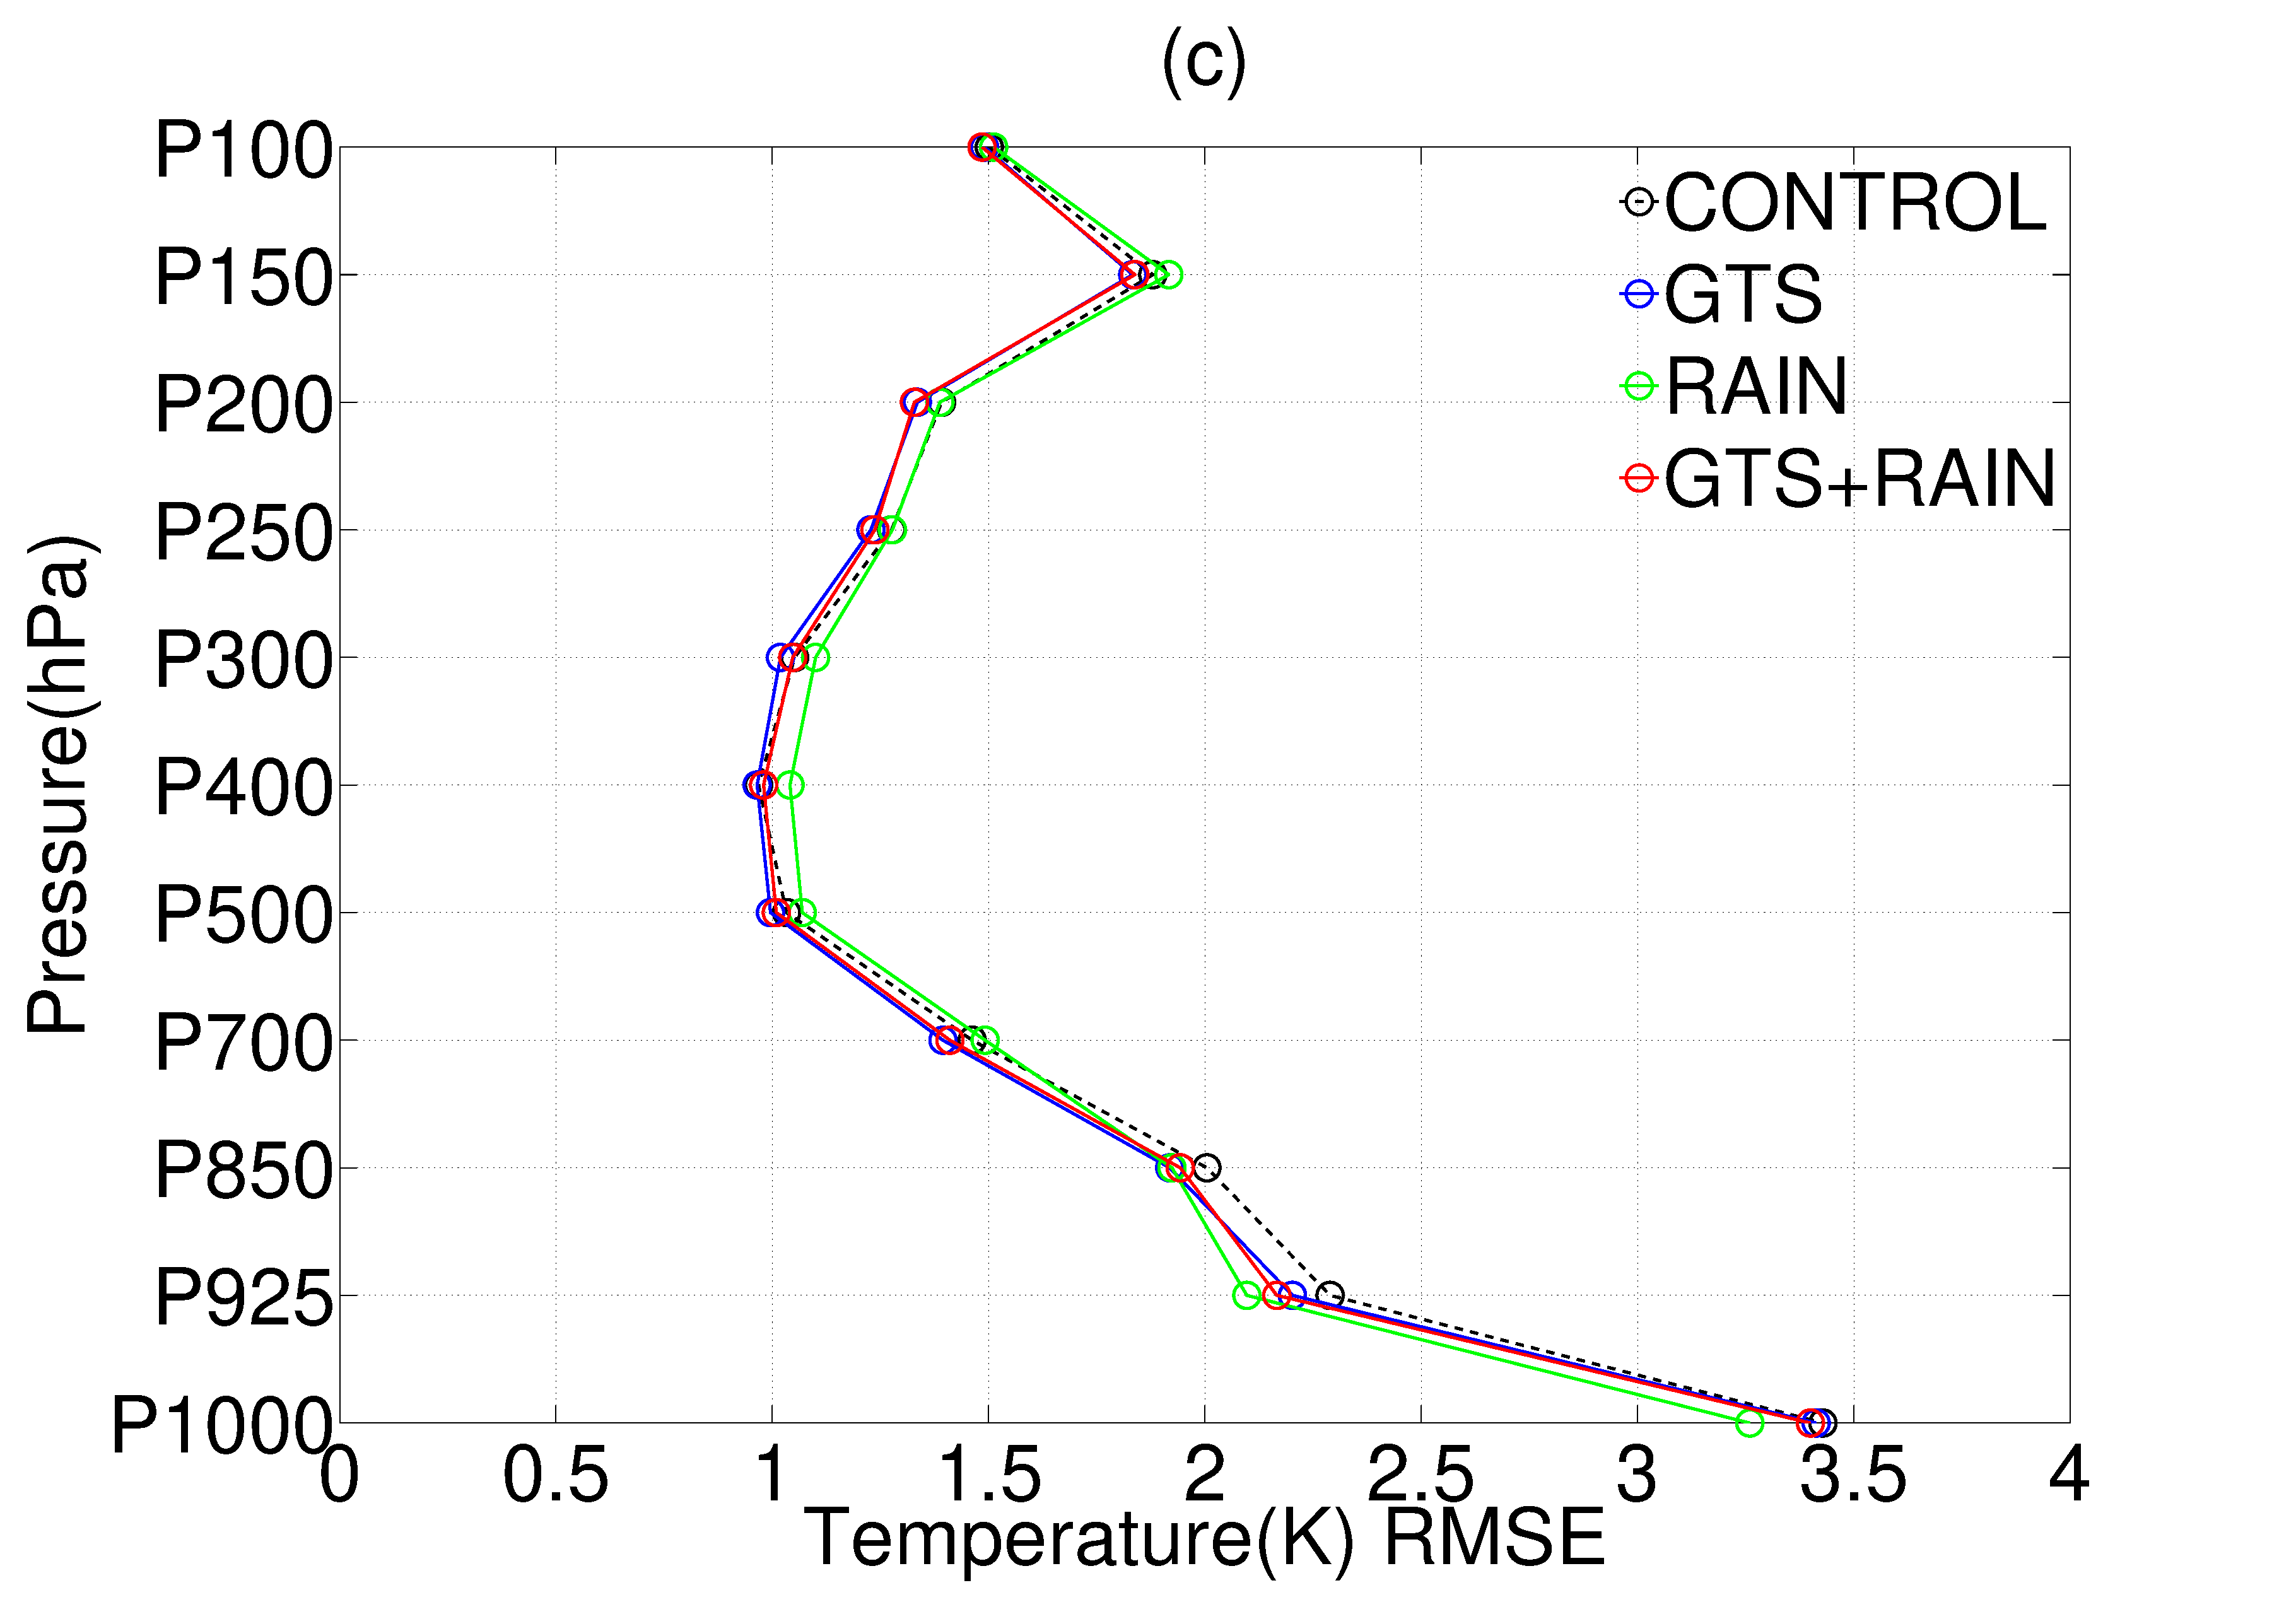
\includegraphics[width=0.5\linewidth]{./figures/tmp_24.eps}
\caption{Same as Figure 1 but for temperature. }\label{tmp_00}
\end{figure}

\newpage
\begin{figure}
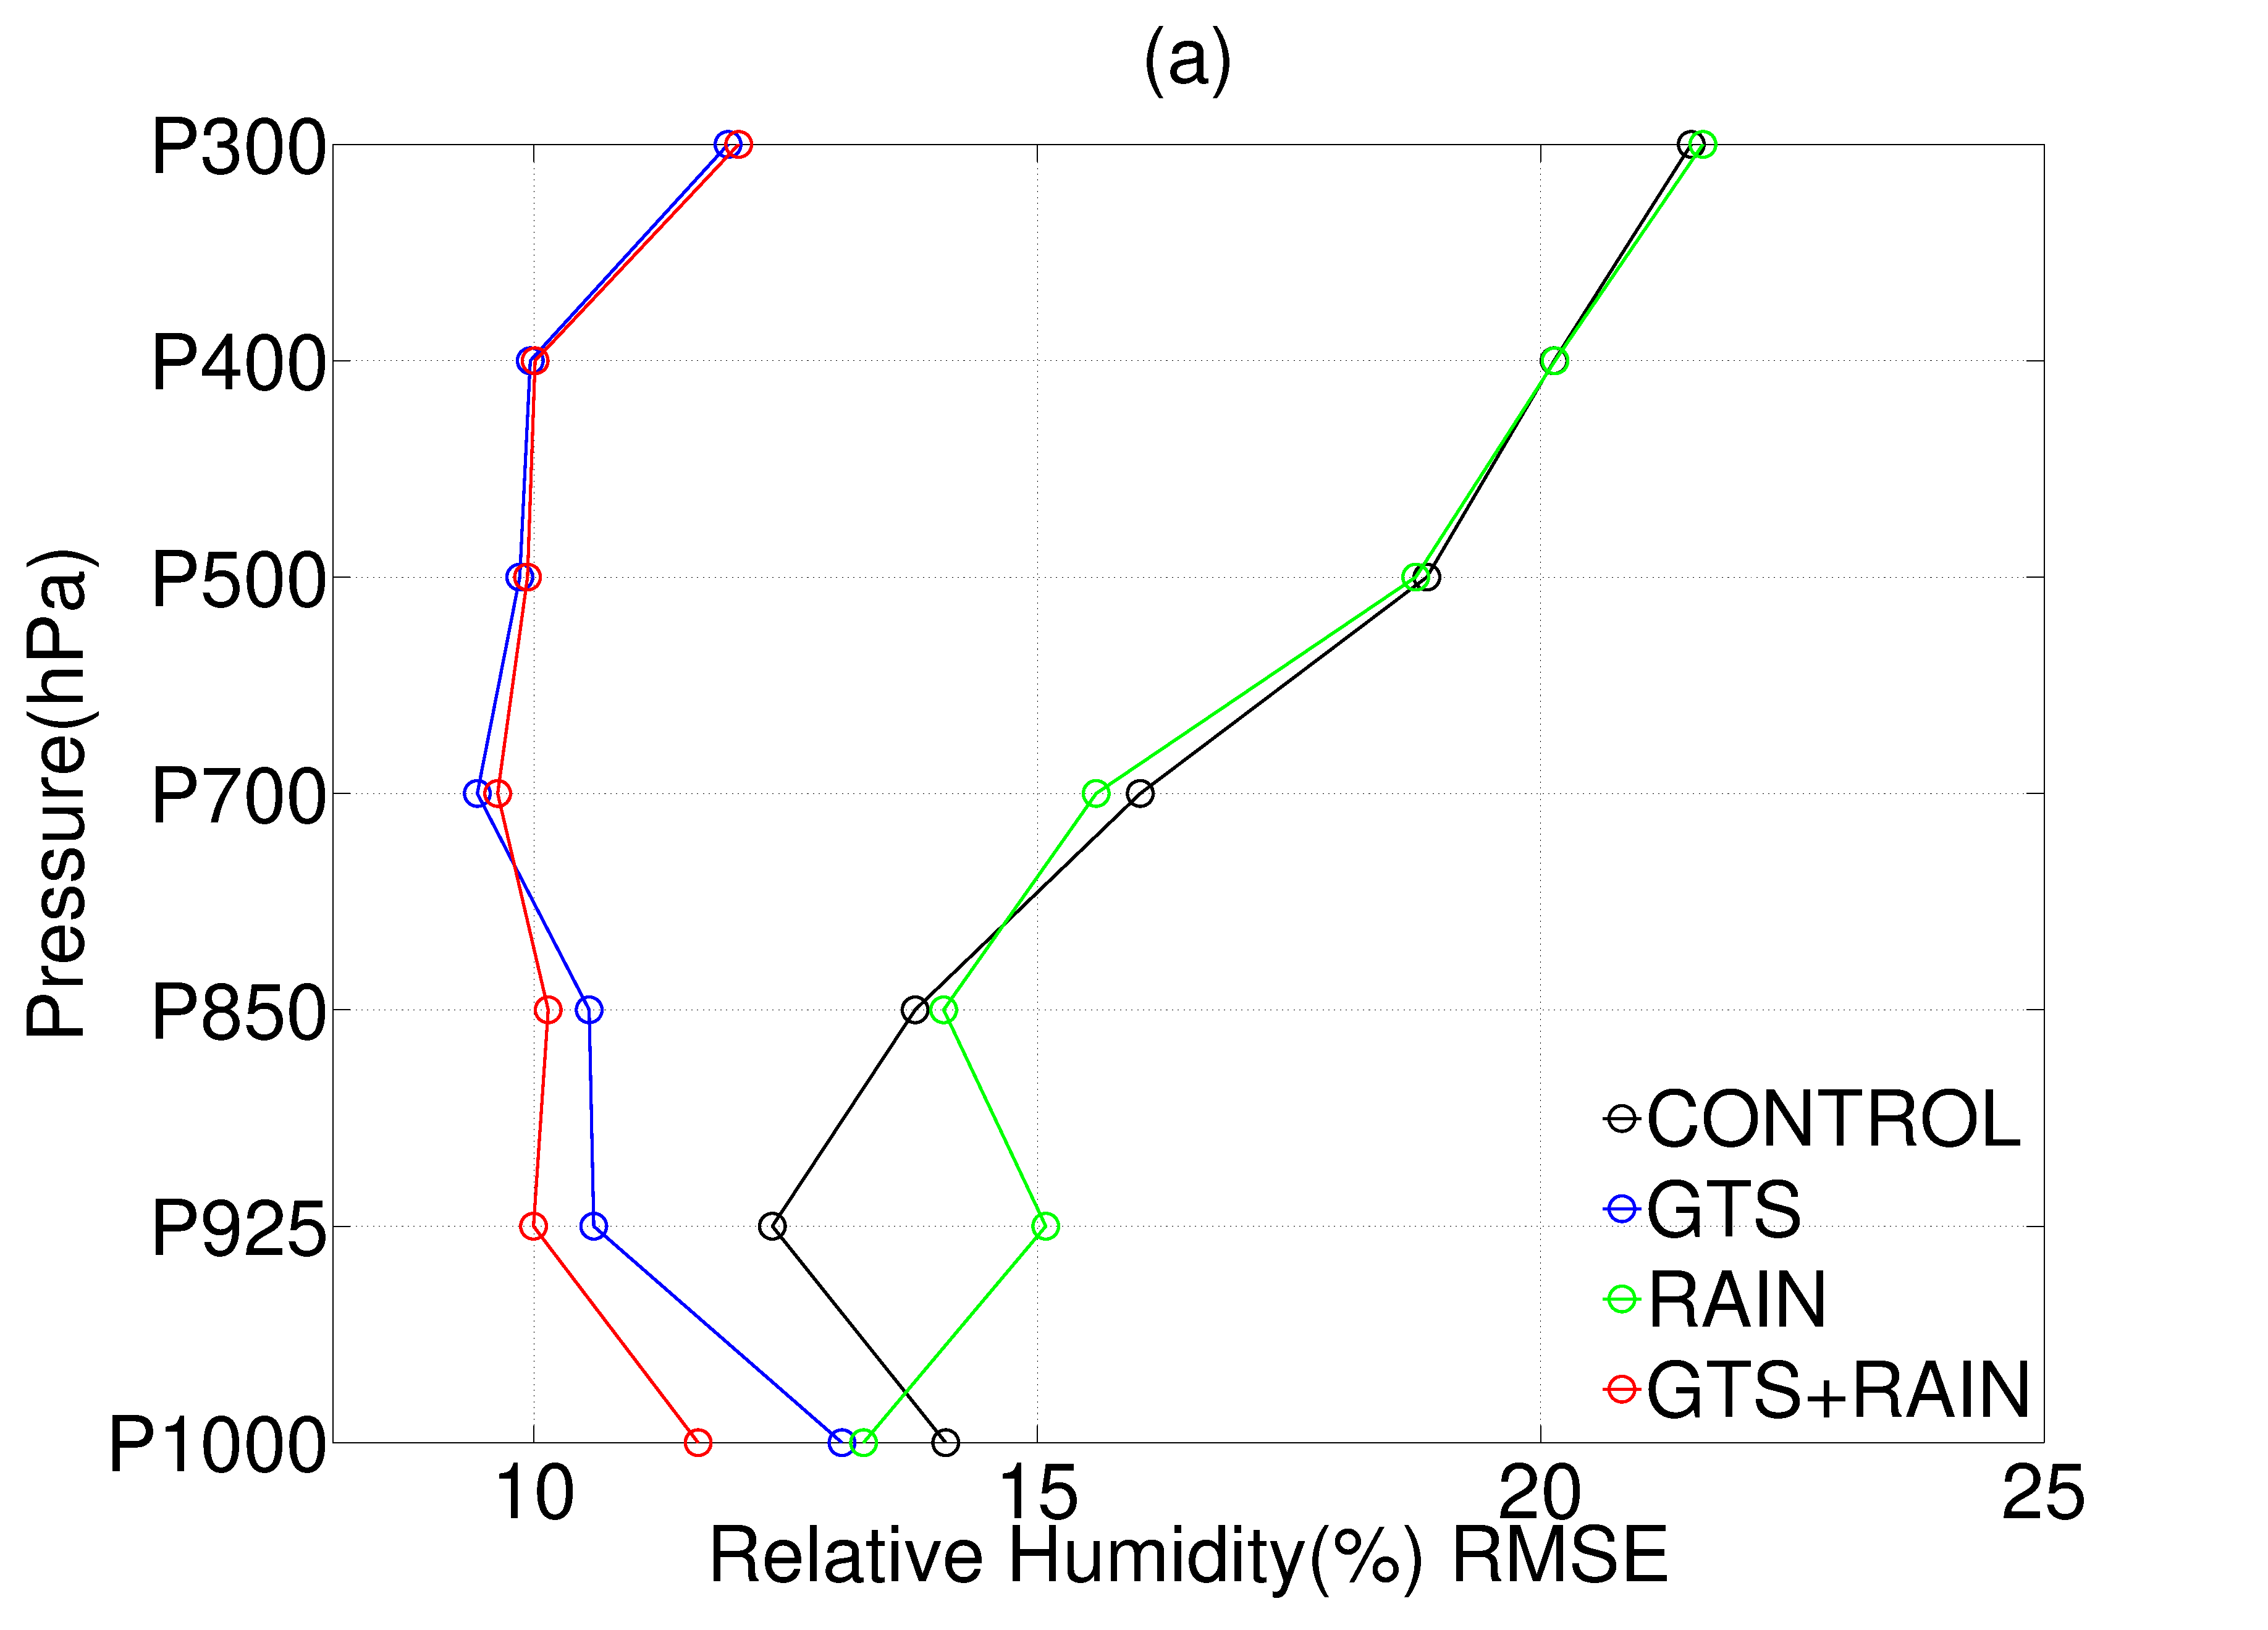
\includegraphics[width=0.5\linewidth]{./figures/rh_00.eps}

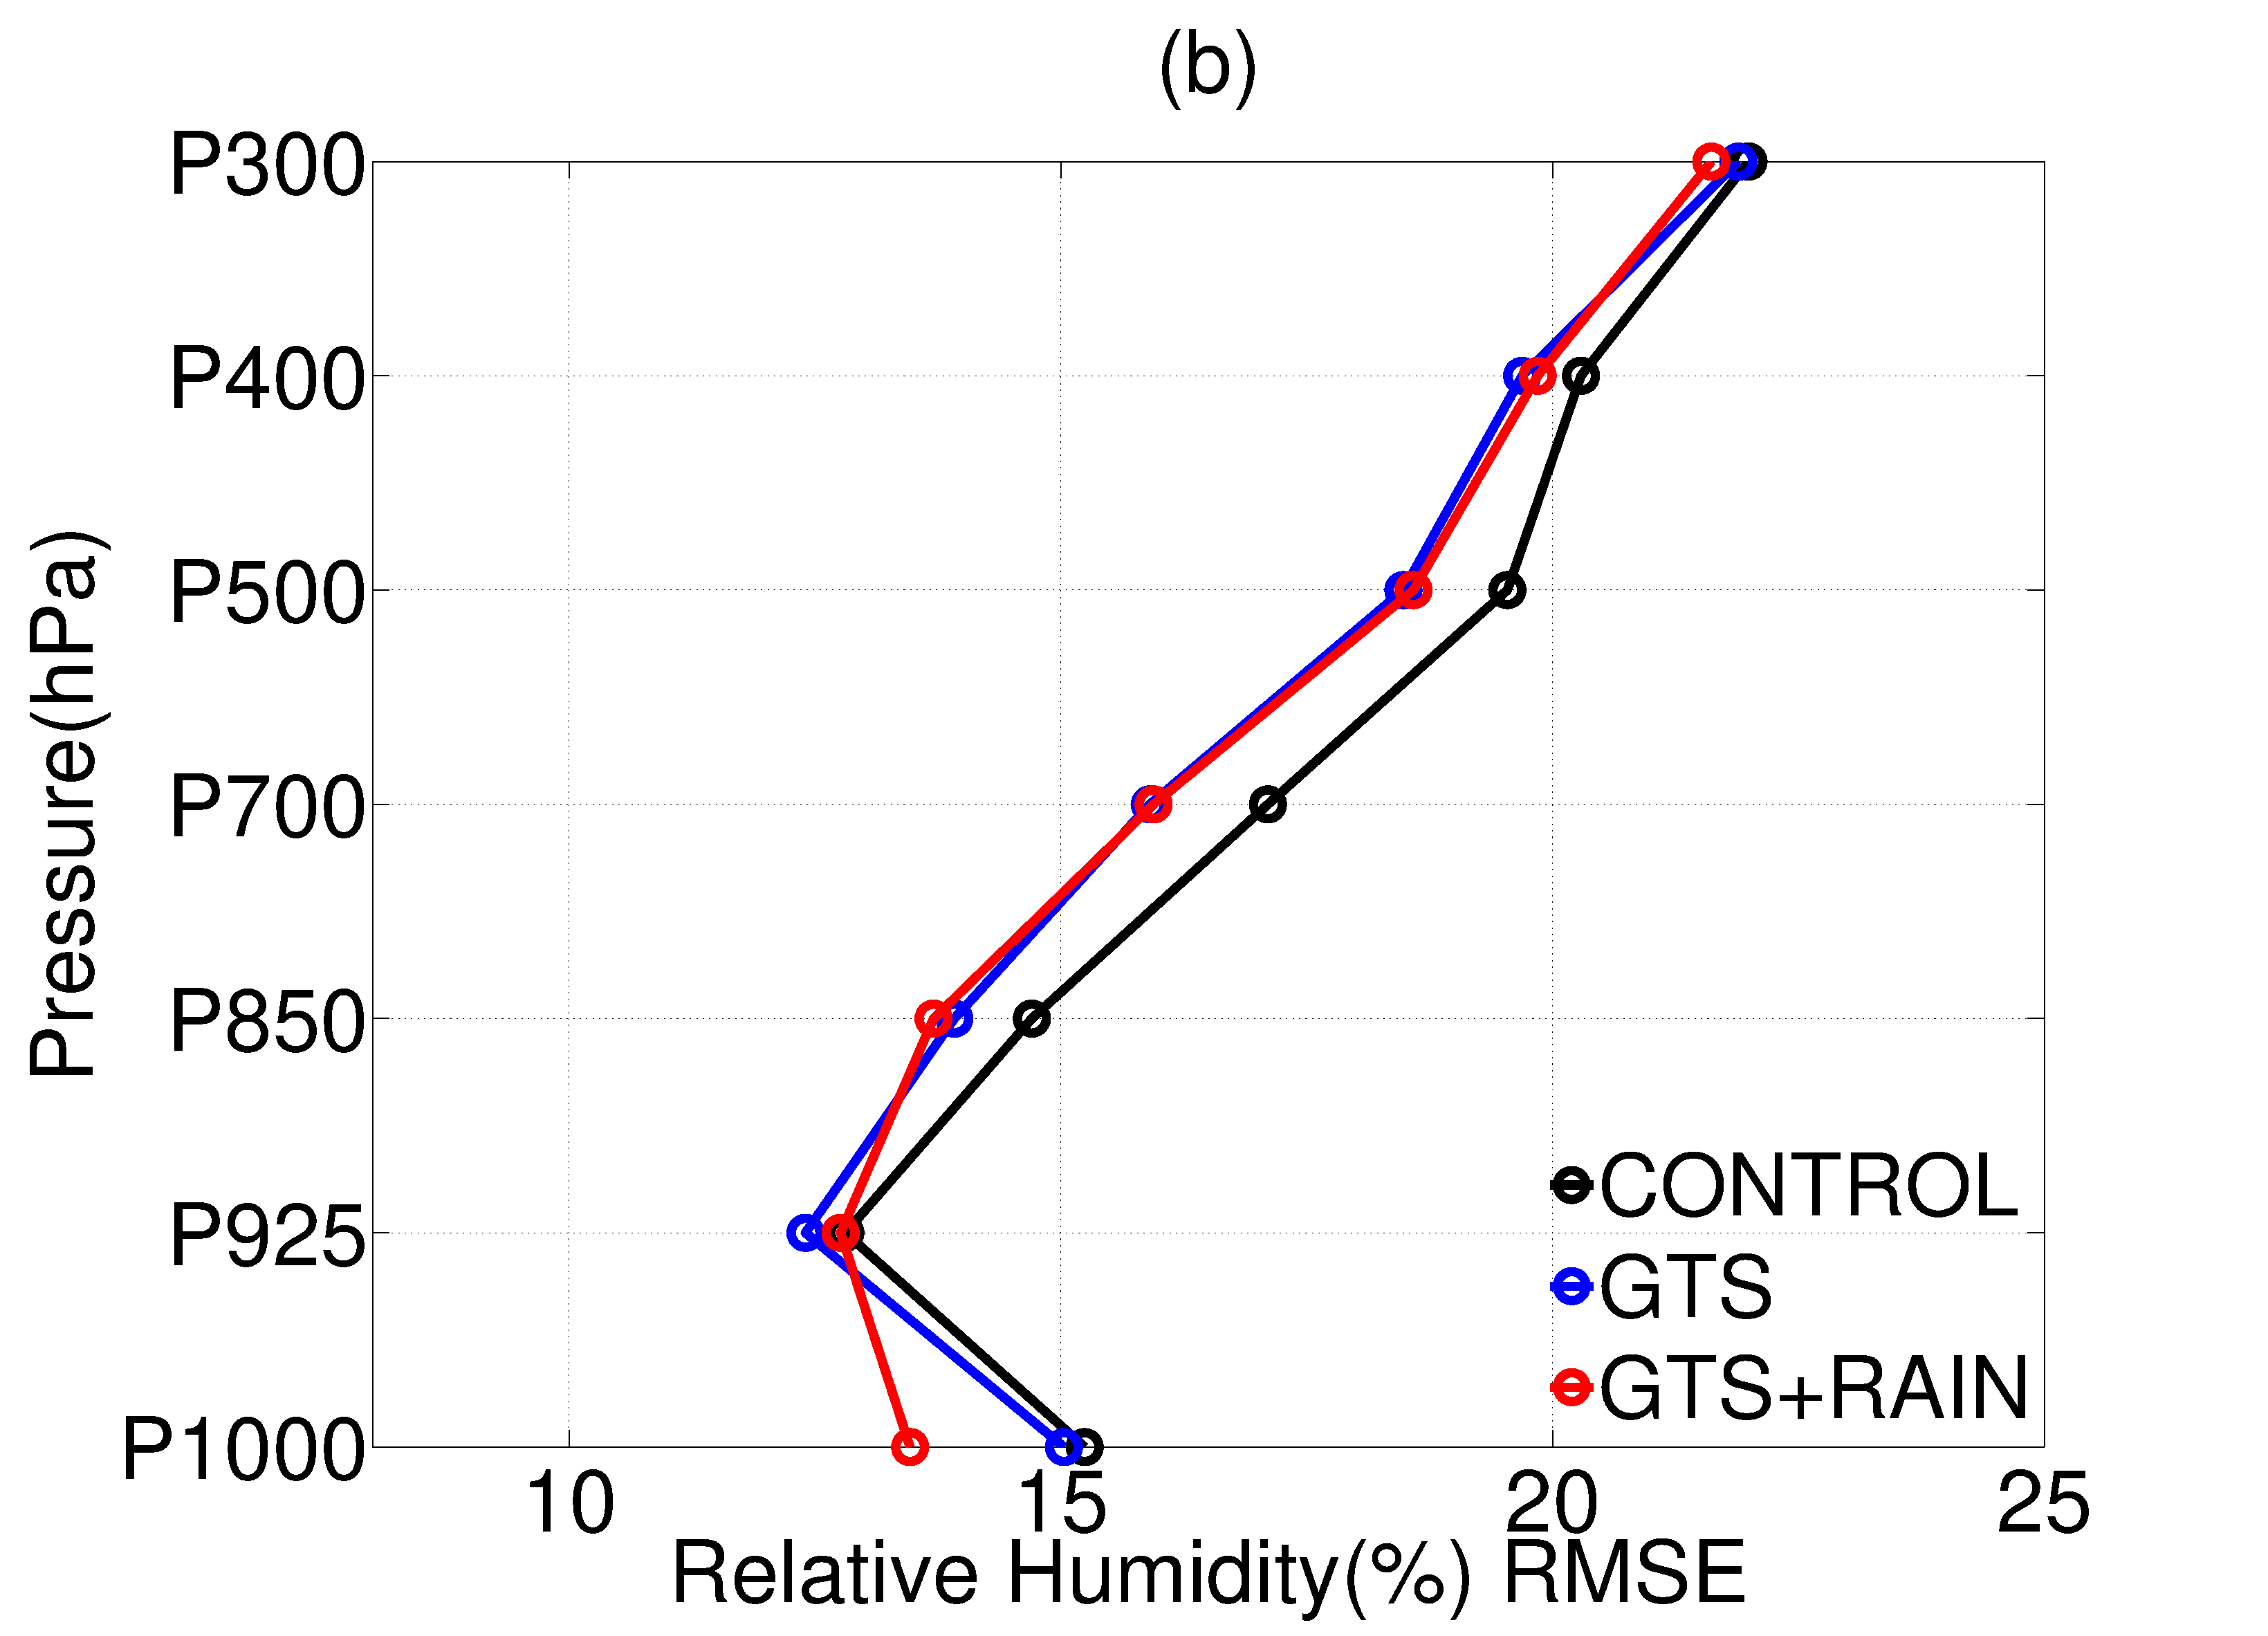
\includegraphics[width=0.5\linewidth]{./figures/rh_12.eps}

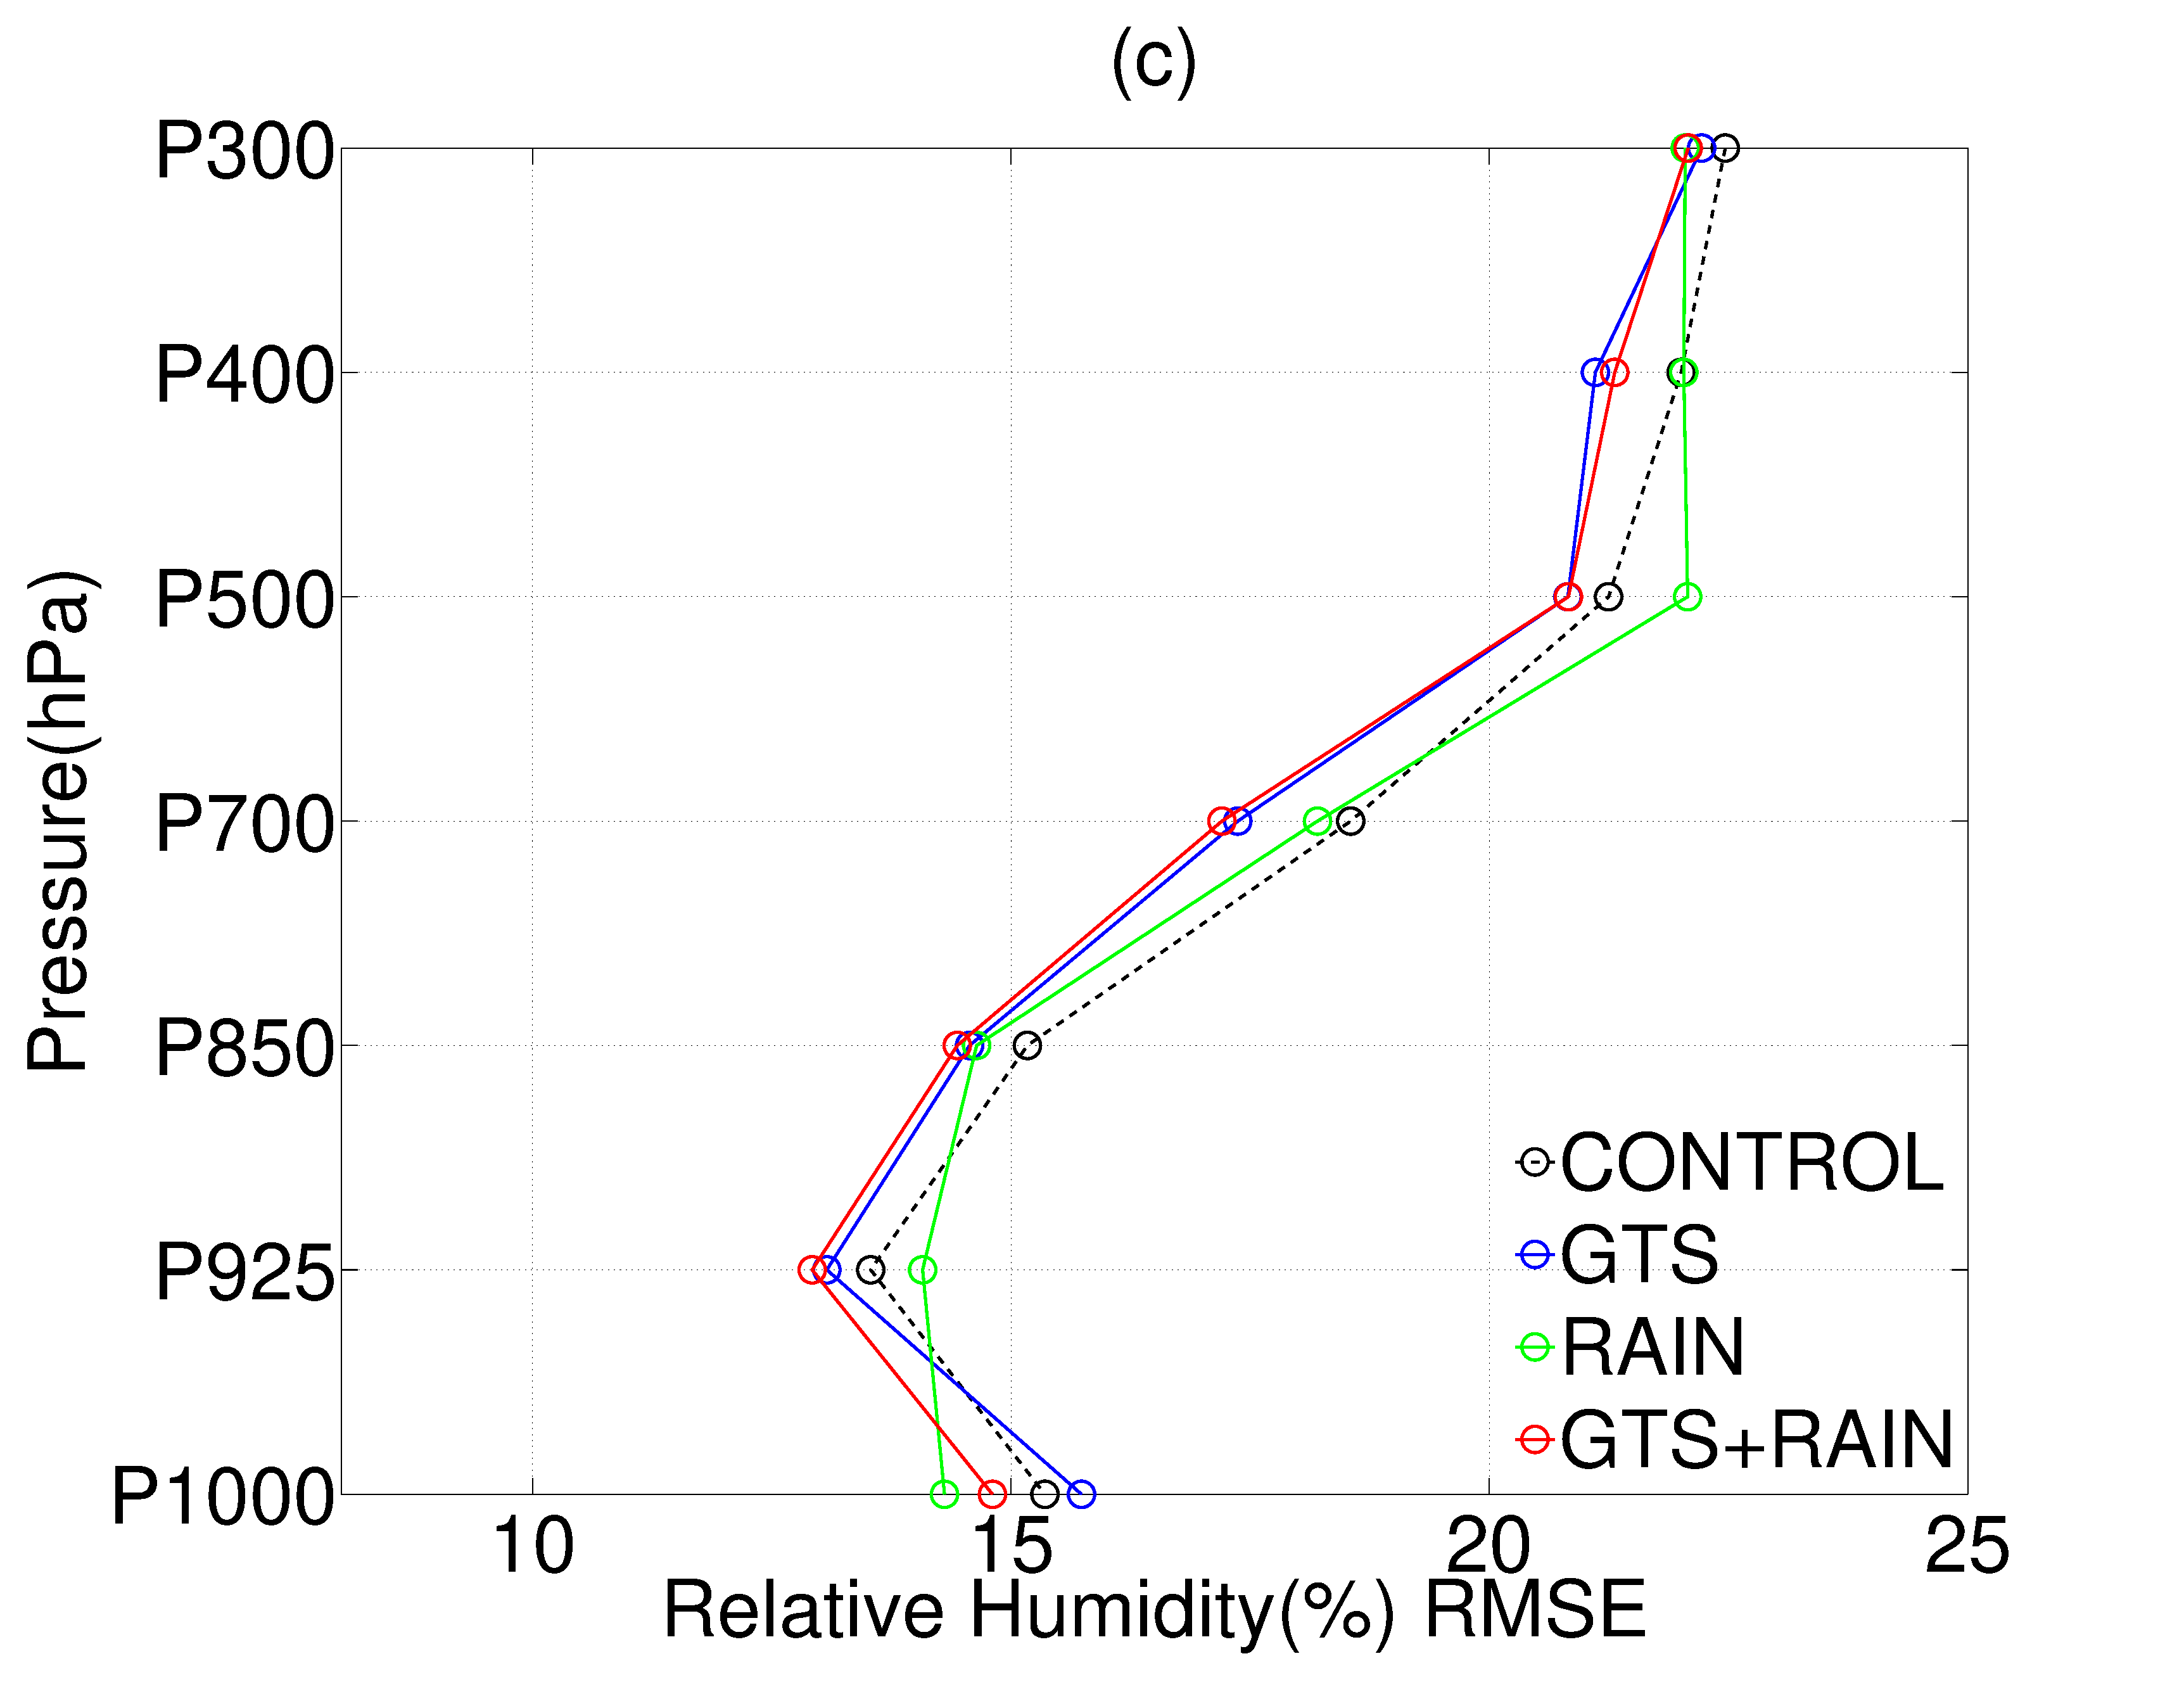
\includegraphics[width=0.5\linewidth]{./figures/rh_24.eps}
\caption{Same as Figure 1 but for relative humidity.}\label{rh_00}
\end{figure}

\newpage
\begin{figure}
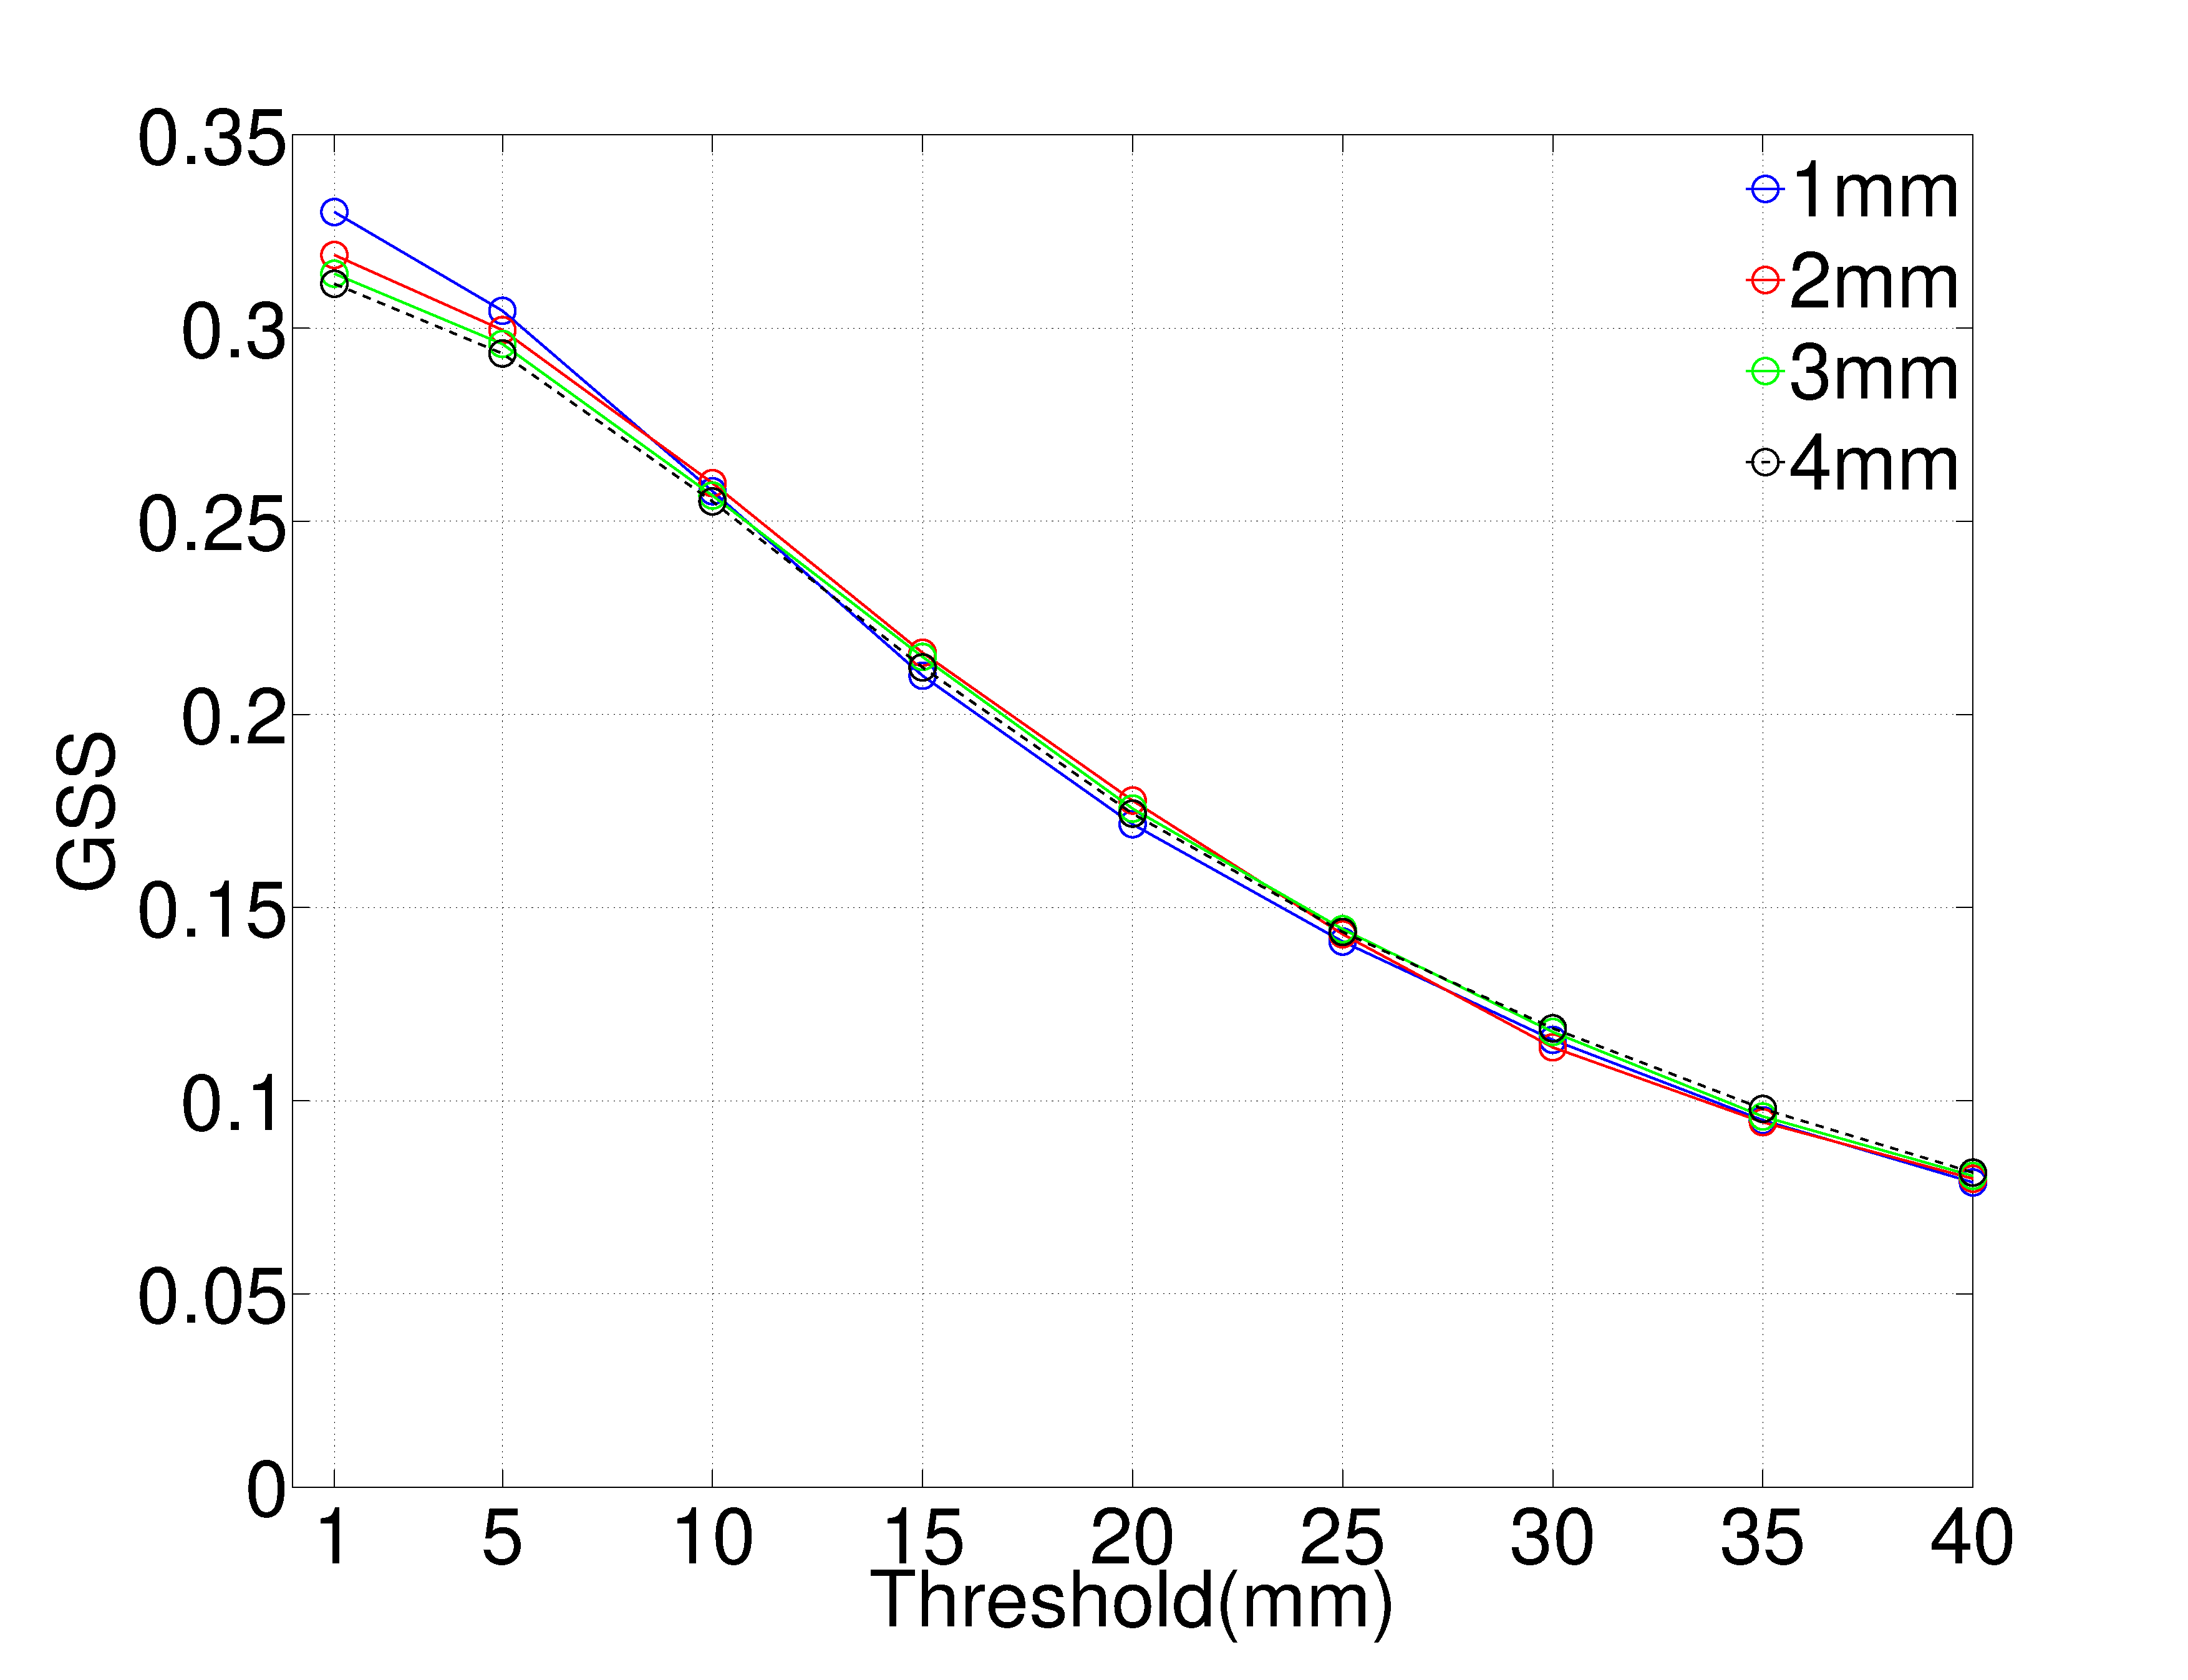
\includegraphics[width=0.5\linewidth]{./figures/gss_24h_error.eps}
\caption{Threshold series of the GSS for 24-h accumulated precipitation using 1mm, 2mm, 3mm and 4mm precipitation observation error respectively.}\label{obserror_test}
\end{figure}

\newpage
\begin{figure}
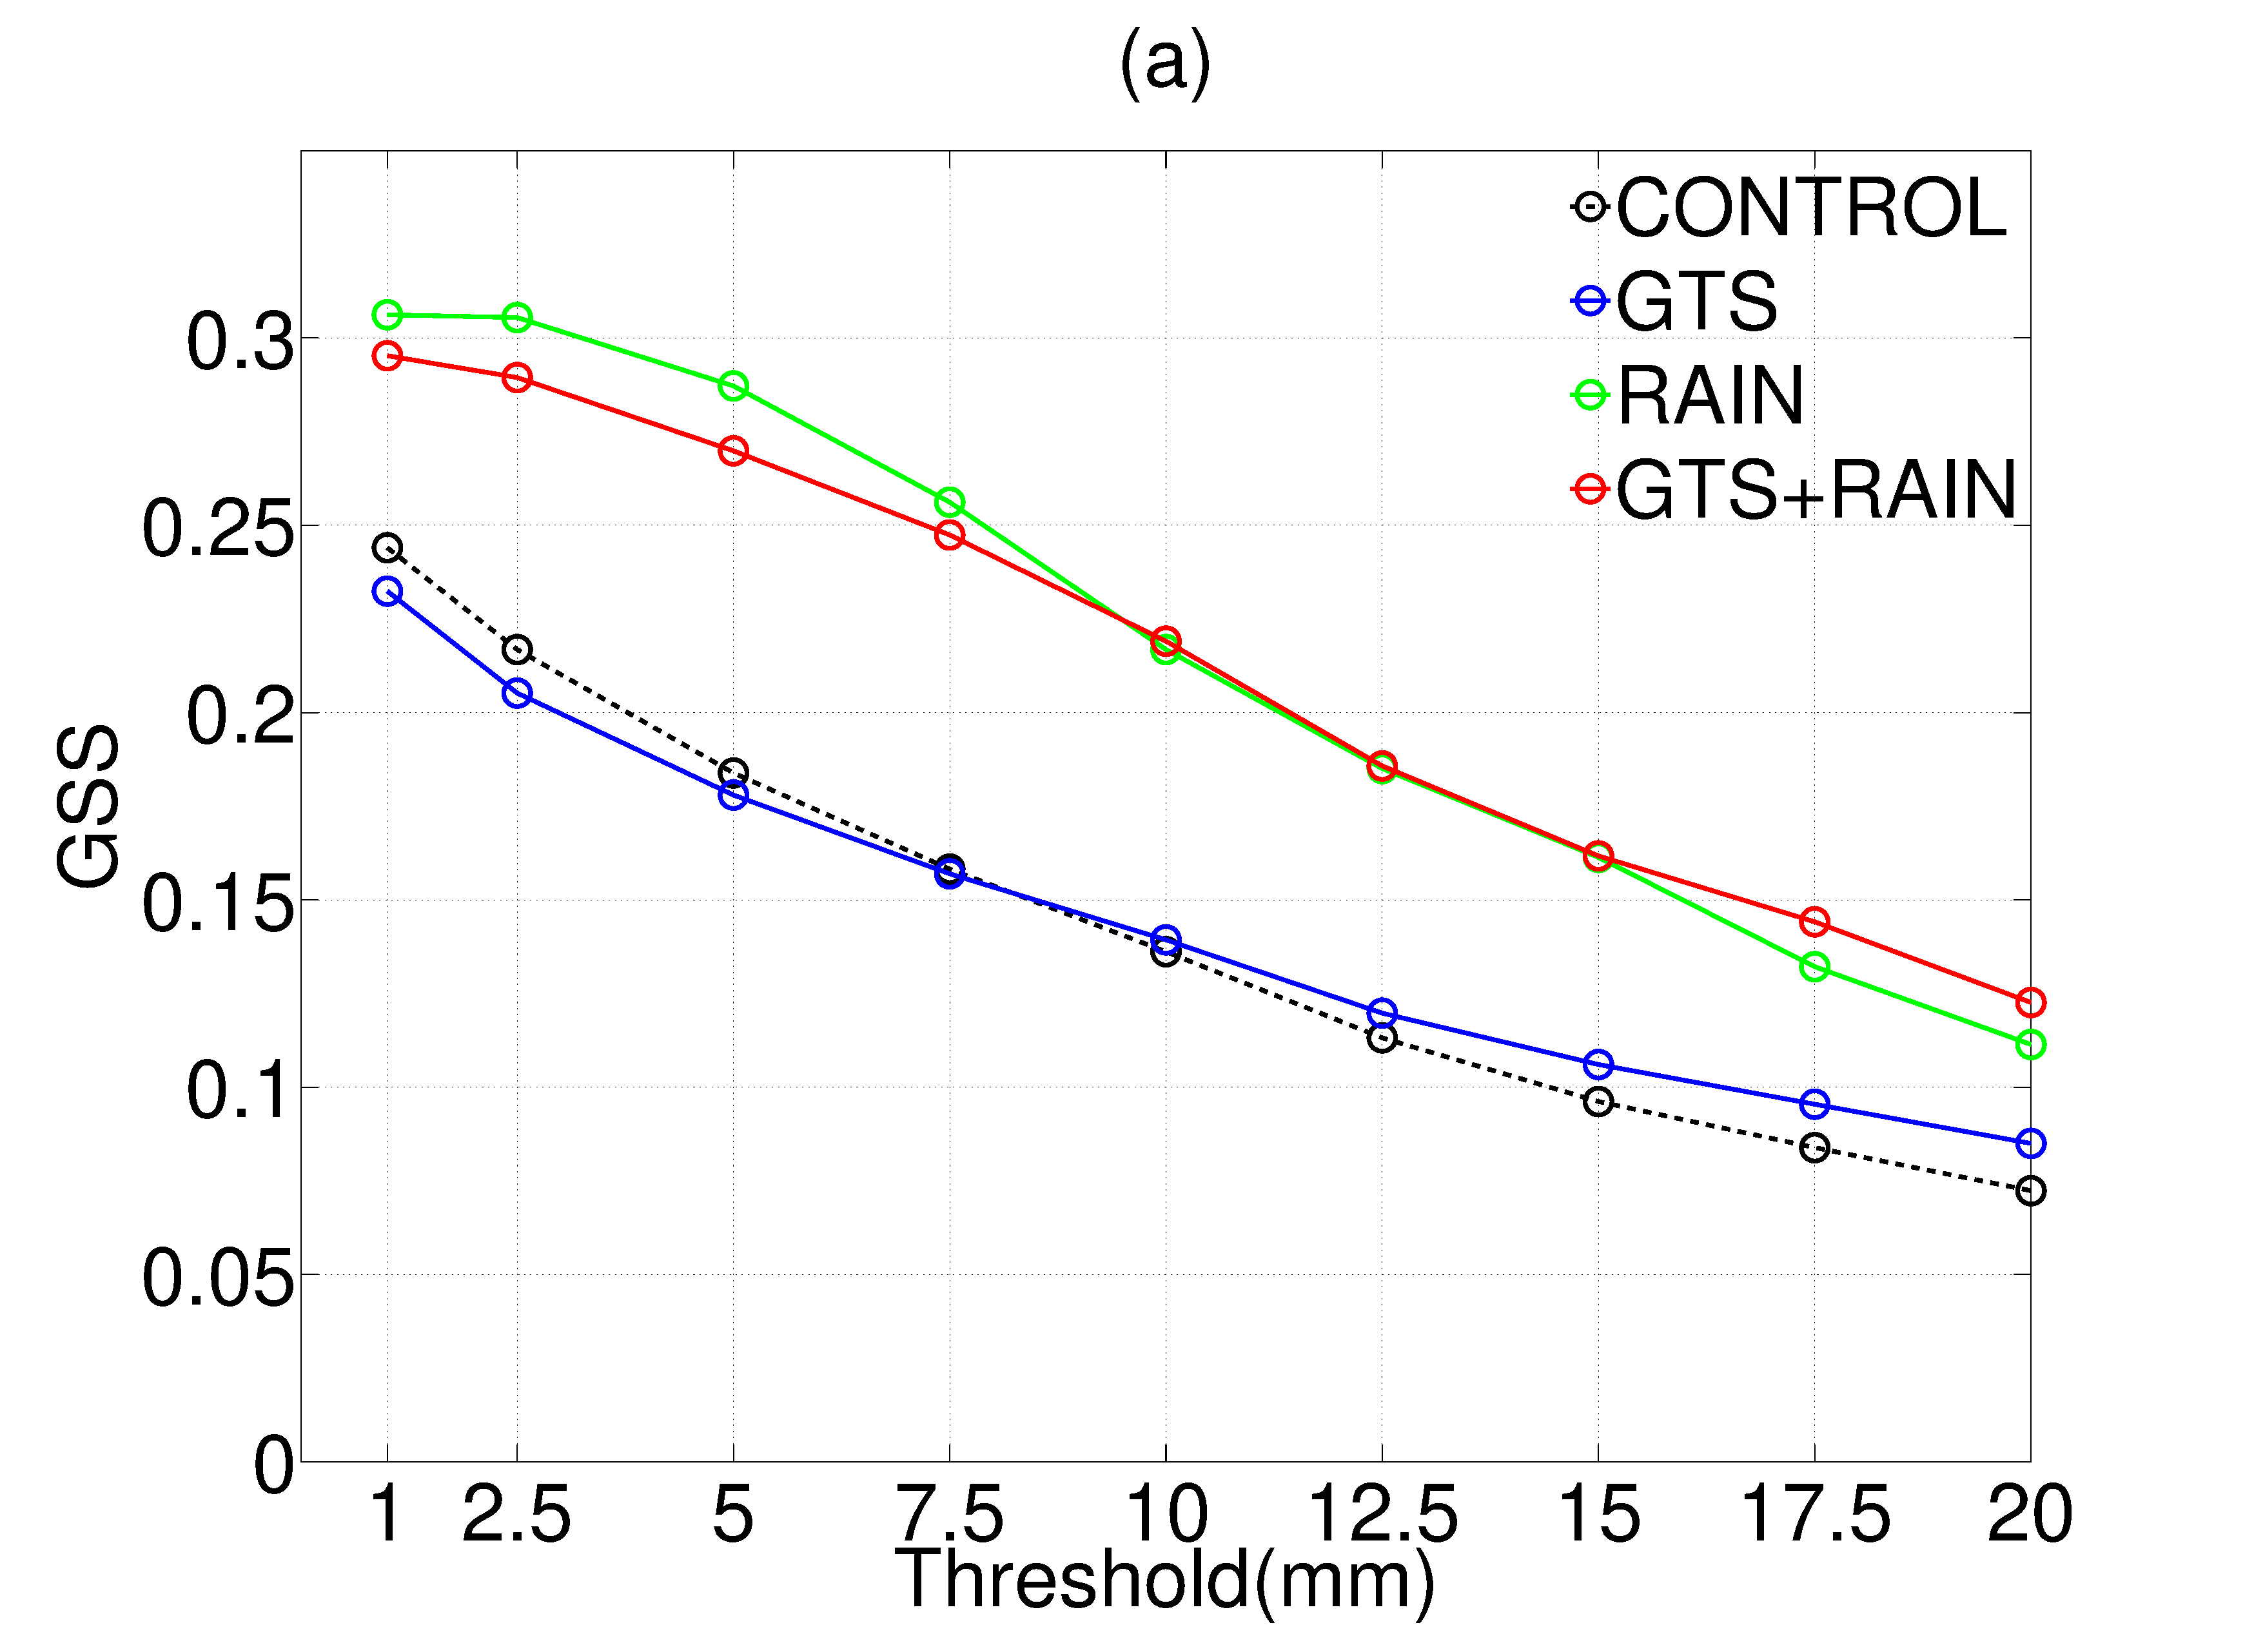
\includegraphics[width=0.5\linewidth]{./figures/GSS_06.eps}
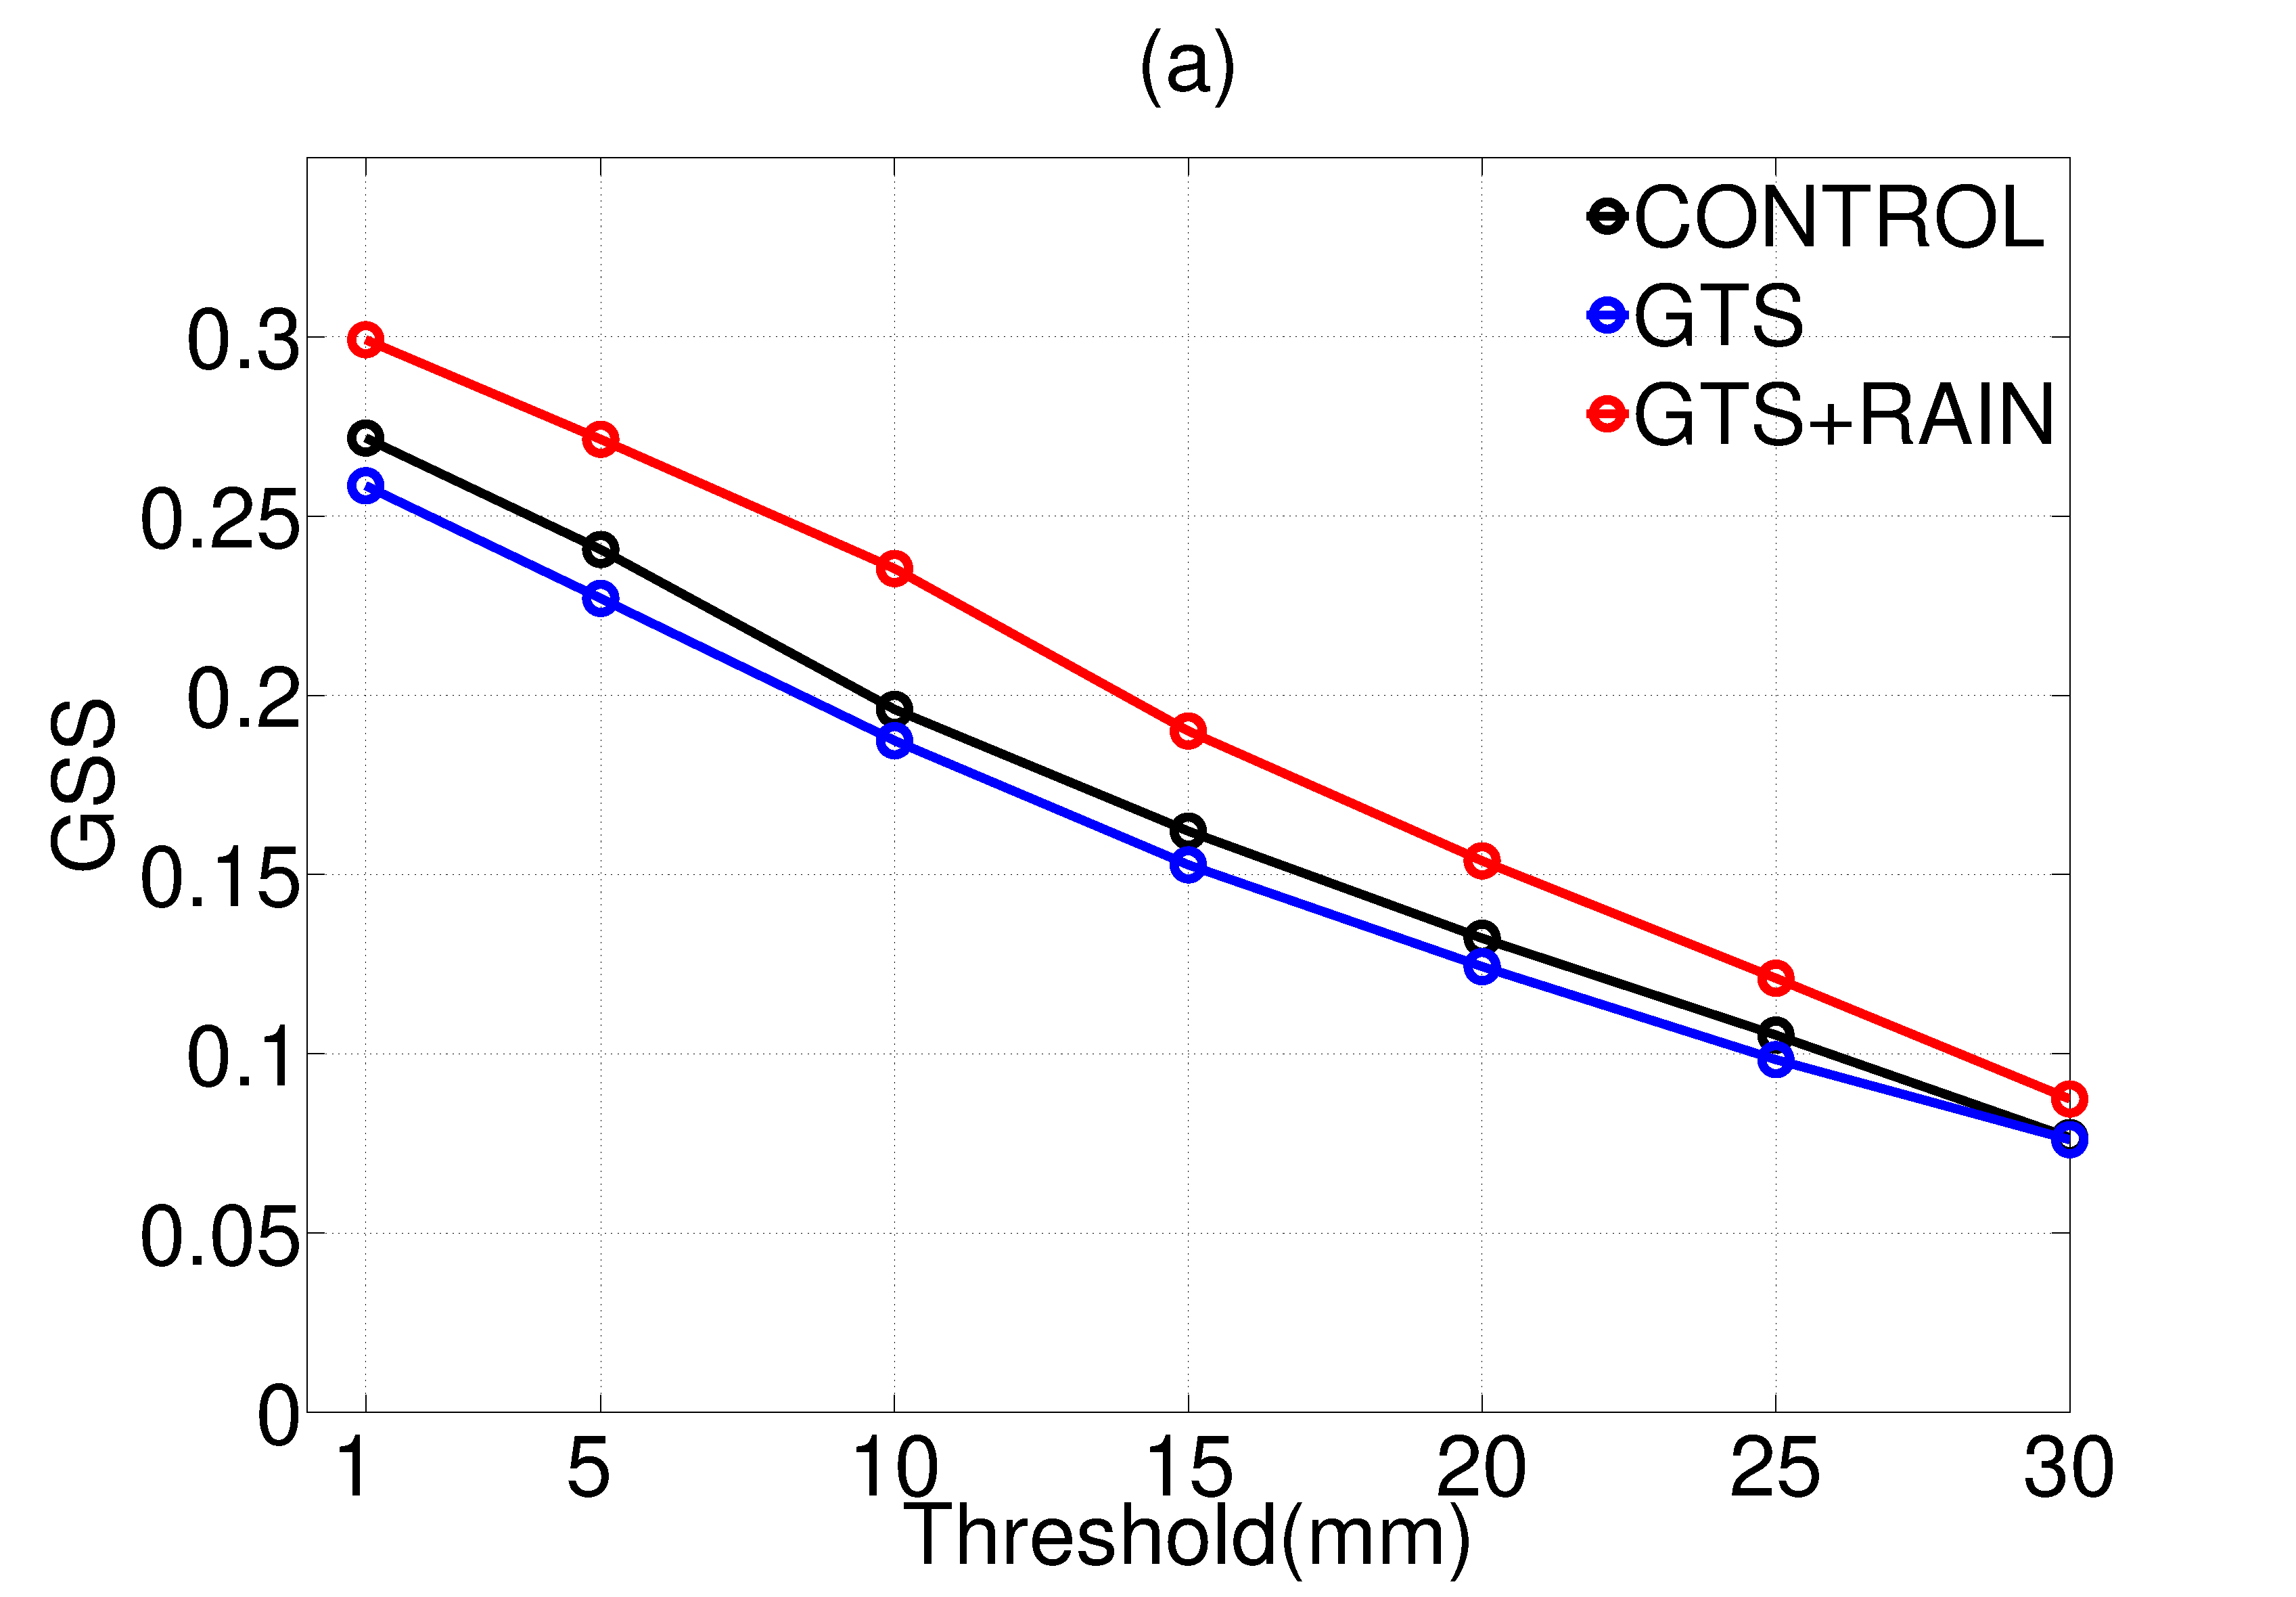
\includegraphics[width=0.5\linewidth]{./figures/GSS_12.eps}
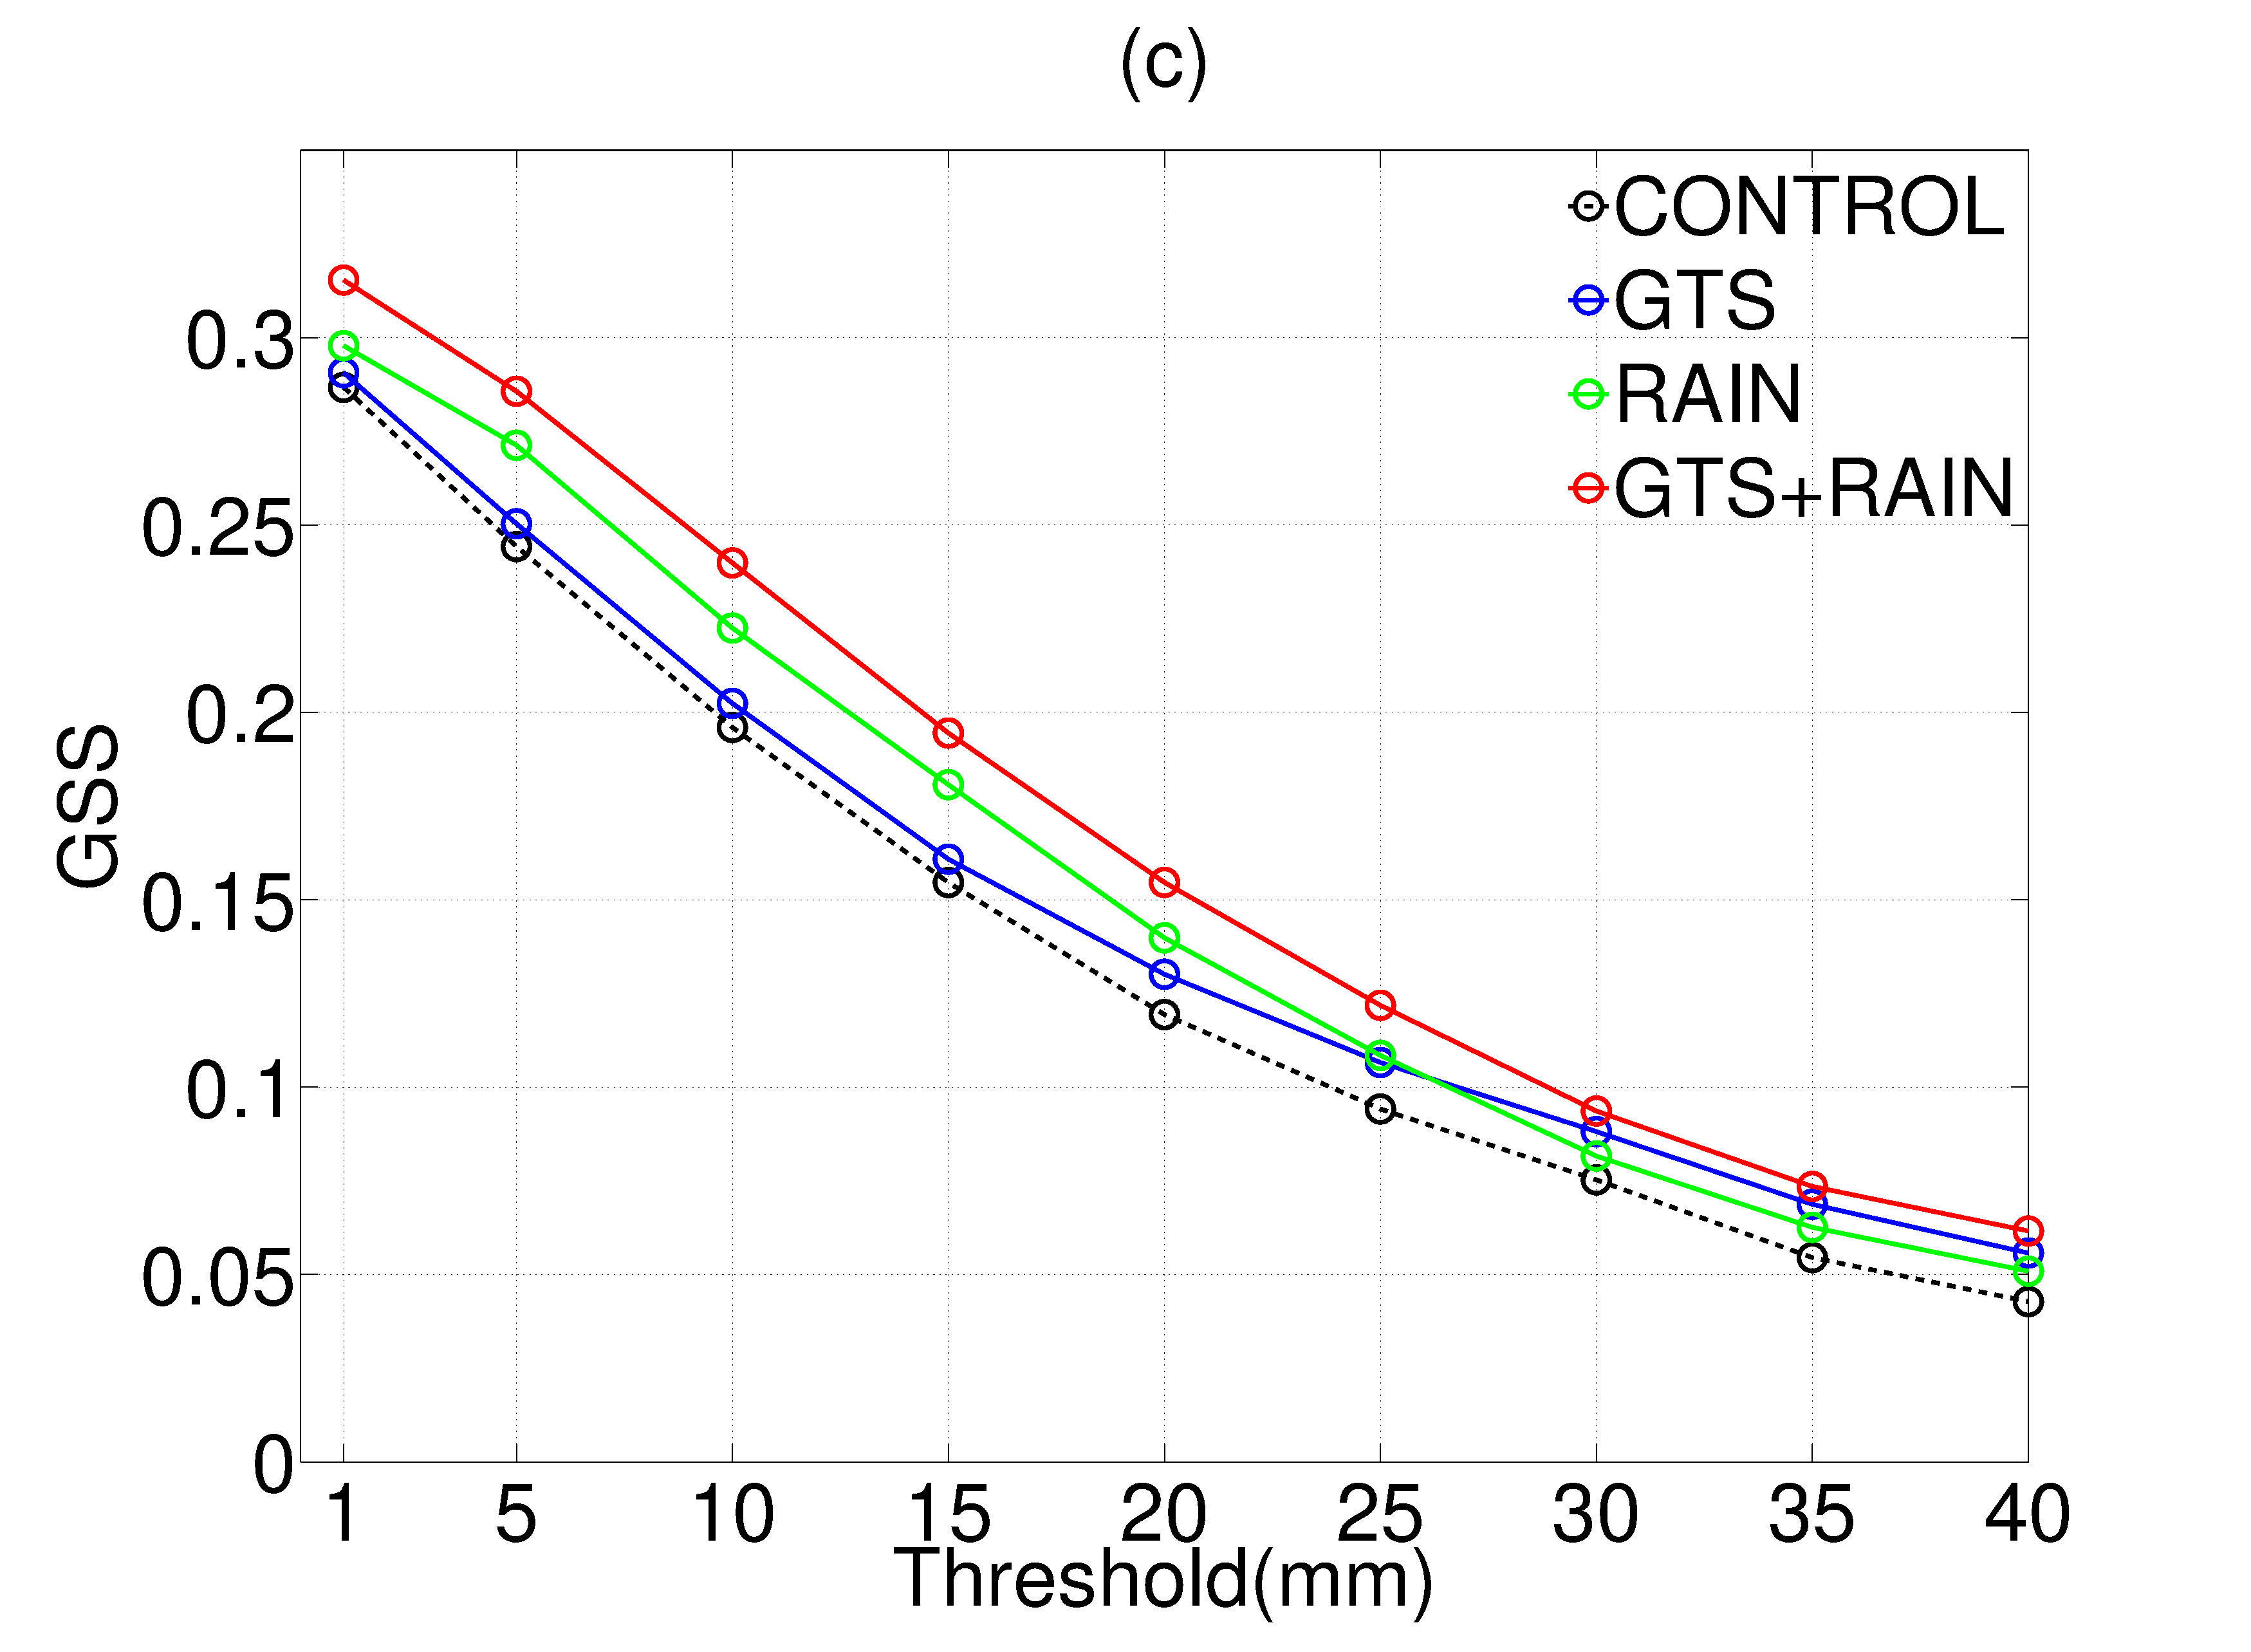
\includegraphics[width=0.5\linewidth]{./figures/GSS_18.eps}
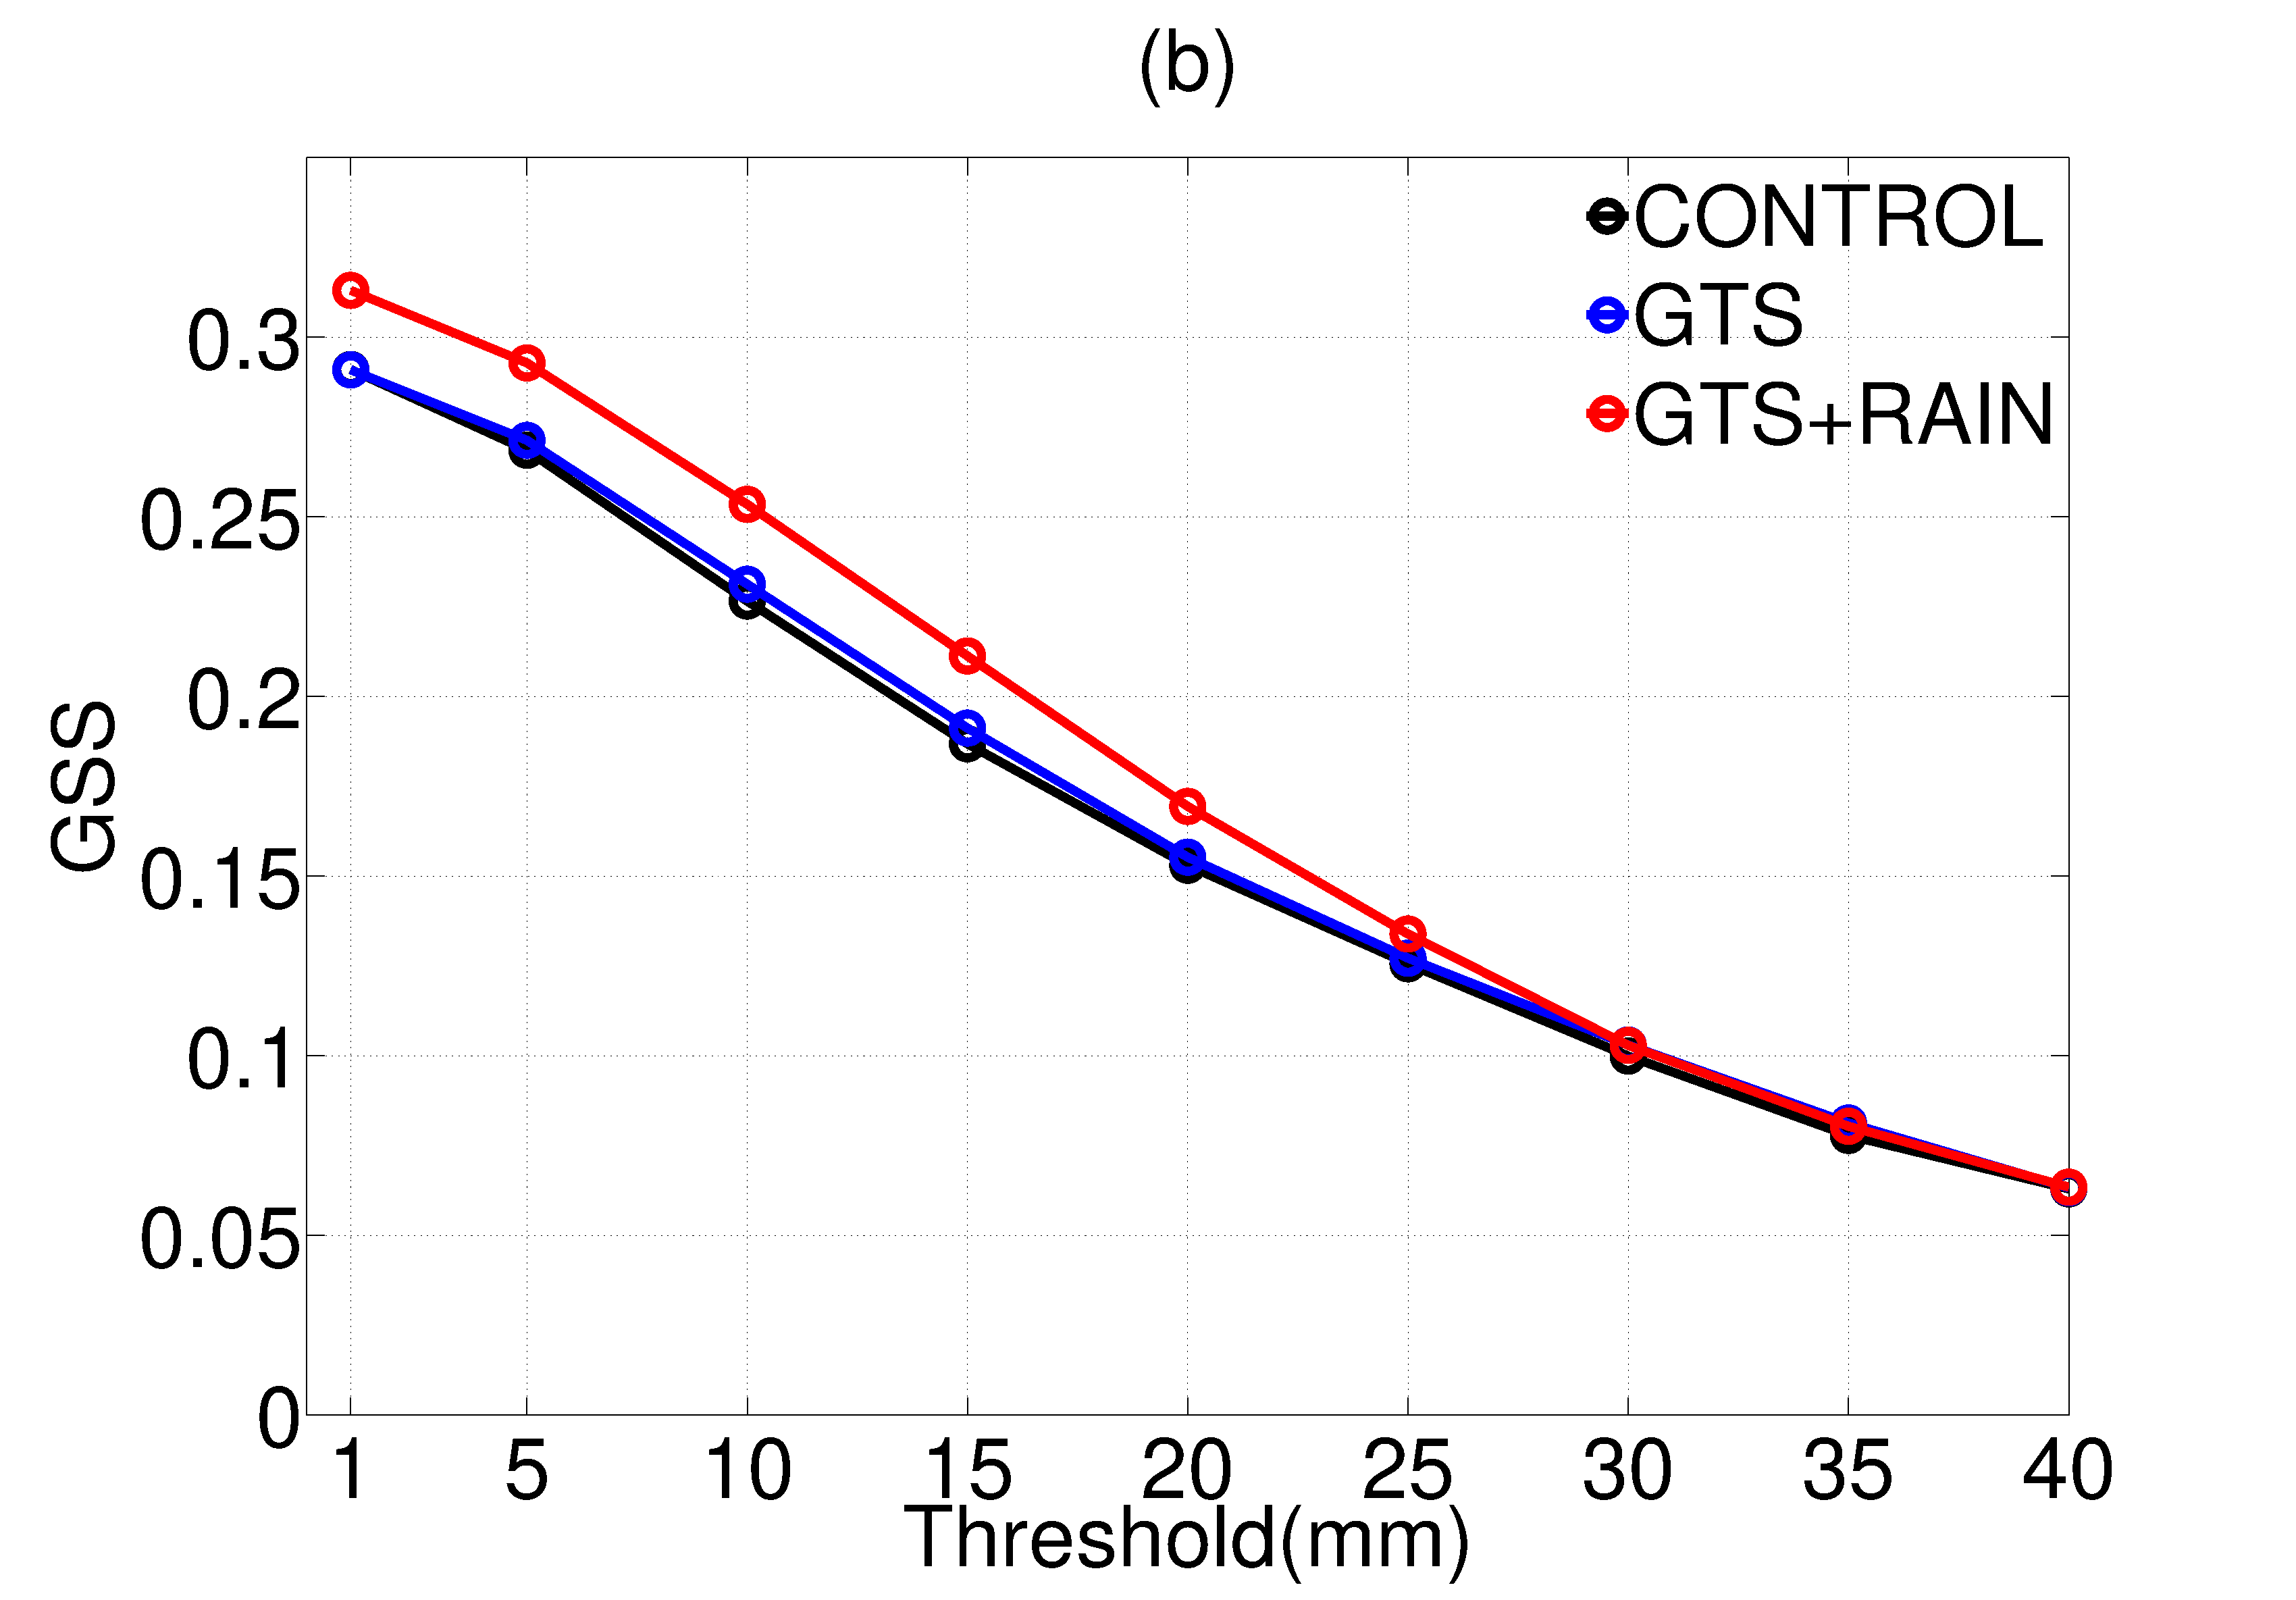
\includegraphics[width=0.5\linewidth]{./figures/GSS_24.eps}
\caption{Threshold series of the GSS for 6-h (a), 12-h (b), 18-h (c), and 24-h (d) accumulated precipitation from the experiment CONTROL, GTS, RAIN, GTS+RAIN. }\label{gss_12h}
\end{figure}

\end{document}

%%%%%%%%%%%%%%%%%%%%%%%%%%%%%%%%%%%%%%%%%%%%%%%%%%%%%%%%%%%%%%%

More Information and Advice:

%% ------------------------------------------------------------------------ %%
%
%  SECTION HEADS
%
%% ------------------------------------------------------------------------ %%

% Capitalize the first letter of each word (except for
% prepositions, conjunctions, and articles that are
% three or fewer letters).

% AGU follows standard outline style; therefore, there cannot be a section 1 without
% a section 2, or a section 2.3.1 without a section 2.3.2.
% Please make sure your section numbers are balanced.
% ---------------
% Level 1 head
%
% Use the \section{} command to identify level 1 heads;
% type the appropriate head wording between the curly
% brackets, as shown below.
%
%An example:
%\section{Level 1 Head: Introduction}
%
% ---------------
% Level 2 head
%
% Use the \subsection{} command to identify level 2 heads.
%An example:
%\subsection{Level 2 Head}
%
% ---------------
% Level 3 head
%
% Use the \subsubsection{} command to identify level 3 heads
%An example:
%\subsubsection{Level 3 Head}
%
%---------------
% Level 4 head
%
% Use the \subsubsubsection{} command to identify level 3 heads
% An example:
%\subsubsubsection{Level 4 Head} An example.
%
%% ------------------------------------------------------------------------ %%
%
%  IN-TEXT LISTS
%
%% ------------------------------------------------------------------------ %%
%
% Do not use bulleted lists; enumerated lists are okay.
% \begin{enumerate}
% \item
% \item
% \item
% \end{enumerate}
%
%% ------------------------------------------------------------------------ %%
%
%  EQUATIONS
%
%% ------------------------------------------------------------------------ %%

% Single-line equations are centered.
% Equation arrays will appear left-aligned.

Math coded inside display math mode \[ ...\]
 will not be numbered, e.g.,:
 \[ x^2=y^2 + z^2\]

 Math coded inside \begin{equation} and \end{equation} will
 be automatically numbered, e.g.,:
 \begin{equation}
 x^2=y^2 + z^2
 \end{equation}

% IF YOU HAVE MULTI-LINE EQUATIONS, PLEASE
% BREAK THE EQUATIONS INTO TWO OR MORE LINES
% OF SINGLE COLUMN WIDTH (20 pc, 8.3 cm)
% using double backslashes (\\).

% To create multiline equations, use the
% \begin{eqnarray} and \end{eqnarray} environment
% as demonstrated below.
\begin{eqnarray}
  x_{1} & = & (x - x_{0}) \cos \Theta \nonumber \\
        && + (y - y_{0}) \sin \Theta  \nonumber \\
  y_{1} & = & -(x - x_{0}) \sin \Theta \nonumber \\
        && + (y - y_{0}) \cos \Theta.
\end{eqnarray}

%If you don't want an equation number, use the star form:
%\begin{eqnarray*}...\end{eqnarray*}

% Break each line at a sign of operation
% (+, -, etc.) if possible, with the sign of operation
% on the new line.

% Indent second and subsequent lines to align with the first character following the equal sign on the first line.

% Use an \hspace{} command to insert horizontal space into your equation if necessary. Place an appropriate unit of measure between the curly braces, e.g. \hspace{1in}; you may have to experiment to achieve the correct amount of space.


%% ------------------------------------------------------------------------ %%
%
%  EQUATION NUMBERING: COUNTER
%
%% ------------------------------------------------------------------------ %%

% You may change equation numbering by resetting
% the equation counter or by explicitly numbering
% an equation.

% To explicitly number an equation, type \eqnum{}
% (with the desired number between the brackets)
% after the \begin{equation} or \begin{eqnarray}
% command.  The \eqnum{} command will affect only
% the equation it appears with; LaTeX will number
% any equations appearing later in the manuscript
% according to the equation counter.
%

% If you have a multiline equation that needs only
% one equation number, use a \nonumber command in
% front of the double backslashes (\\) as shown in
% the multiline equation above.

%% ------------------------------------------------------------------------ %%
%
%  SIDEWAYS FIGURE AND TABLE EXAMPLES
%
%% ------------------------------------------------------------------------ %%
%
% For tables and figures, add \usepackage{rotating} to the paper and add the rotating.sty file to the folder.
% AGU prefers the use of {sidewaystable} over {landscapetable} as it causes fewer problems.
%
% \begin{sidewaysfigure}
% \includegraphics[width=20pc]{samplefigure.eps}
% \caption{caption here}
% \label{label_here}
% \end{sidewaysfigure}
%
% \begin{sidewaystable}
% \caption{}
% \begin{tabular}
% Table layout here.
% \end{tabular}
% \end{sidewaystable}